% =========================================================
% CAPÍTULO 5: ANÁLISIS DEL SISTEMA
% Cada sección vive en su carpeta 5.X_<nombre>/ con su
% seccion5_X.tex (contenido) y seccion5_X.bib (referencias).
% Las columnas K y Q de las tablas de 5.1.2 y 5.2 se definen
% en setup/settings.tex.
% =========================================================

% =========================================================
% 5.1 REQUERIMIENTOS
% =========================================================
\section{Requerimientos}
\label{sec:requerimientos}
Los requerimientos de esta sección se presentan de forma individual, de manera que cada uno describe una sola función del sistema y puede comprobarse mediante al menos un criterio de aceptación. Las reglas del negocio que afectan a varios requerimientos, como el área de servicio, los catálogos, las vigencias y los umbrales, se establecen una sola vez en la sección \textit{Reglas del negocio} y se indican mediante su identificador cuando sea necesario.


\subsection{Requerimientos funcionales}
% =========================================================
% Requerimientos funcionales en formato de tabla
% Requiere \input{rf_tablas_preambulo} en el preámbulo.
% Orden de argumentos de \tablaRF:
%   {Identificador}{Nombre}{Prioridad}{Requerimiento}
%   {Entrada}{Salida}{Descripción}{Precondición}{Postcondición}
% =========================================================
En esta sección se definen los requerimientos que requiere el software para cumplir con la norma IEEE/ISO/IEC 29148-2018\cite{iso29148}, la cual es la guía sobre cómo descubrir, redactar y estructurar los requerimientos desde el inicio del proyecto.

\subsubsection{Autenticación y cuenta}

\tablaRF{RF-01}% Identificador
  {Registro de cuenta con correo electrónico}% Nombre
  {Alta}% Prioridad
  {El sistema permite que el usuario registre una cuenta con su correo electrónico y una contraseña.}% Requerimiento
  {Correo electrónico y contraseña}% Entrada
  {Cuenta registrada pendiente de verificación}% Salida
  {El sistema debe permitir que el usuario registre una cuenta proporcionando correo electrónico y contraseña.}% Descripción
  {El correo electrónico no debe estar asociado a otra cuenta registrada.}% Precondición
  {La cuenta queda registrada en estado no verificado.}% Postcondición

\tablaRF{RF-02}% Identificador
  {Verificación del correo electrónico}% Nombre
  {Alta}% Prioridad
  {El sistema permite verificar el correo electrónico registrado mediante un enlace.}% Requerimiento
  {Correo electrónico proporcionado en el registro}% Entrada
  {Correo con enlace de verificación}% Salida
  {El sistema debe enviar un enlace de verificación al correo electrónico proporcionado durante el registro, conforme a RN-17.}% Descripción
  {El usuario debe haber registrado una cuenta con correo electrónico y contraseña.}% Precondición
  {El enlace queda enviado al correo del usuario y, al abrirse, la cuenta queda verificada.}% Postcondición

\tablaRF{RF-03}% Identificador
  {Restricción de cuentas no verificadas}% Nombre
  {Alta}% Prioridad
  {El sistema restringe el acceso a la aplicación a las cuentas no verificadas.}% Requerimiento
  {Intento de acceso con una cuenta no verificada}% Entrada
  {Acceso denegado y aviso de verificación pendiente}% Salida
  {El sistema debe restringir el acceso a las funciones de la aplicación mientras la cuenta no esté verificada.}% Descripción
  {La cuenta del usuario debe estar registrada sin haber sido verificada.}% Precondición
  {Las funciones de la aplicación permanecen bloqueadas hasta que la cuenta se verifique.}% Postcondición

\tablaRF{RF-04}% Identificador
  {Inicio de sesión con correo electrónico}% Nombre
  {Alta}% Prioridad
  {El sistema permite iniciar sesión con correo electrónico y contraseña.}% Requerimiento
  {Correo electrónico y contraseña}% Entrada
  {Sesión iniciada}% Salida
  {El sistema debe permitir que el usuario inicie sesión mediante correo electrónico y contraseña.}% Descripción
  {El usuario debe contar con una cuenta registrada y verificada.}% Precondición
  {La sesión del usuario queda activa y se muestra la pantalla principal.}% Postcondición

\tablaRF{RF-05}% Identificador
  {Autenticación con Google}% Nombre
  {Media}% Prioridad
  {El sistema permite registrarse e iniciar sesión con una cuenta de Google.}% Requerimiento
  {Autorización de la cuenta de Google}% Entrada
  {Cuenta registrada o sesión iniciada}% Salida
  {El sistema debe permitir que el usuario registre una cuenta e inicie sesión mediante una cuenta de Google.}% Descripción
  {El usuario debe contar con una cuenta de Google y el dispositivo debe tener conexión a internet.}% Precondición
  {La sesión del usuario queda activa y vinculada a su cuenta de Google.}% Postcondición

\tablaRF{RF-06}% Identificador
  {Cierre de sesión}% Nombre
  {Media}% Prioridad
  {El sistema permite que el usuario cierre su sesión.}% Requerimiento
  {Selección de la opción de cerrar sesión en el menú principal}% Entrada
  {Sesión finalizada}% Salida
  {El sistema debe permitir que el usuario autenticado cierre su sesión desde el menú principal.}% Descripción
  {El usuario debe tener una sesión iniciada.}% Precondición
  {La sesión queda cerrada y se muestra la pantalla de inicio de sesión.}% Postcondición

\tablaRF{RF-07}% Identificador
  {Cambio de contraseña}% Nombre
  {Media}% Prioridad
  {El sistema permite que el usuario cambie su contraseña.}% Requerimiento
  {Contraseña vigente y nueva contraseña}% Entrada
  {Contraseña actualizada}% Salida
  {El sistema debe permitir que el usuario autenticado cambie su contraseña, solicitando la contraseña vigente.}% Descripción
  {El usuario debe tener una sesión iniciada con una cuenta de correo electrónico y contraseña.}% Precondición
  {La nueva contraseña queda registrada y la anterior deja de ser válida.}% Postcondición

\tablaRF{RF-08}% Identificador
  {Recuperación de contraseña}% Nombre
  {Media}% Prioridad
  {El sistema permite recuperar la contraseña mediante un enlace enviado al correo electrónico.}% Requerimiento
  {Correo electrónico de la cuenta}% Entrada
  {Correo con enlace de restablecimiento}% Salida
  {El sistema debe permitir que el usuario solicite la recuperación de su contraseña mediante un enlace de restablecimiento enviado a su correo electrónico, sujeto a RN-14.}% Descripción
  {El usuario debe contar con una cuenta registrada con correo electrónico y contraseña.}% Precondición
  {El enlace de restablecimiento queda enviado al correo del usuario.}% Postcondición

\tablaRF{RF-09}% Identificador
  {Eliminación de cuenta}% Nombre
  {Media}% Prioridad
  {El sistema permite que el usuario elimine su cuenta.}% Requerimiento
  {Solicitud de eliminación y confirmación explícita}% Entrada
  {Cuenta eliminada}% Salida
  {El sistema debe permitir que el usuario elimine su cuenta, aplicando el tratamiento de datos descrito en RN-15 y solicitando confirmación explícita antes de ejecutar la eliminación.}% Descripción
  {El usuario debe tener una sesión iniciada.}% Precondición
  {La cuenta queda eliminada y sus datos reciben el tratamiento descrito en RN-15.}% Postcondición

\subsubsection{Mapa y visualización}

\tablaRF{RF-10}% Identificador
  {Mapa base interactivo}% Nombre
  {Alta}% Prioridad
  {El sistema muestra un mapa interactivo que responde a gestos táctiles.}% Requerimiento
  {Gestos táctiles de acercamiento, alejamiento y desplazamiento}% Entrada
  {Mapa actualizado conforme al gesto realizado}% Salida
  {El sistema debe mostrar un mapa base interactivo que responda a gestos táctiles de acercamiento, alejamiento y desplazamiento libre.}% Descripción
  {El usuario debe tener una sesión iniciada.}% Precondición
  {El mapa queda visible con el nivel de acercamiento y la posición resultantes del gesto.}% Postcondición

\tablaRF{RF-11}% Identificador
  {Búsqueda de origen y destino}% Nombre
  {Alta}% Prioridad
  {El sistema permite indicar el origen y el destino mediante la búsqueda de direcciones.}% Requerimiento
  {Texto de la dirección buscada}% Entrada
  {Sugerencias de autocompletado y dirección seleccionada}% Salida
  {El sistema debe permitir que el usuario indique su origen y su destino mediante una barra de búsqueda de direcciones con sugerencias de autocompletado.}% Descripción
  {El usuario debe encontrarse en la pantalla del mapa y el dispositivo debe tener conexión a internet.}% Precondición
  {El origen o el destino quedan establecidos en la dirección seleccionada.}% Postcondición

\tablaRF{RF-12}% Identificador
  {Selección de origen y destino en el mapa}% Nombre
  {Media}% Prioridad
  {El sistema permite indicar el origen y el destino seleccionando un punto en el mapa.}% Requerimiento
  {Punto seleccionado sobre el mapa}% Entrada
  {Origen o destino marcado en el mapa}% Salida
  {El sistema debe permitir que el usuario indique su origen y su destino seleccionando manualmente un punto sobre el mapa.}% Descripción
  {El usuario debe encontrarse en la pantalla del mapa.}% Precondición
  {El origen o el destino quedan establecidos en el punto seleccionado.}% Postcondición

\tablaRF{RF-13}% Identificador
  {Gestión de lugares favoritos}% Nombre
  {Baja}% Prioridad
  {El sistema permite administrar lugares favoritos y usarlos como accesos rápidos.}% Requerimiento
  {Ubicación y etiqueta del lugar favorito}% Entrada
  {Lugar favorito creado, editado o eliminado}% Salida
  {El sistema debe permitir que el usuario cree, edite y elimine lugares favoritos identificados con una etiqueta propia, y debe ofrecerlos como accesos rápidos al indicar origen o destino.}% Descripción
  {El usuario debe tener una sesión iniciada.}% Precondición
  {Los lugares favoritos quedan disponibles como accesos rápidos al indicar origen o destino.}% Postcondición

\tablaRF{RF-14}% Identificador
  {Visualización de puntos de ayuda}% Nombre
  {Media}% Prioridad
  {El sistema muestra en el mapa los puntos de ayuda.}% Requerimiento
  {Área visible del mapa}% Entrada
  {Marcadores de puntos de ayuda}% Salida
  {El sistema debe mostrar sobre el mapa, como marcadores, puntos de ayuda.}% Descripción
  {El usuario debe encontrarse en la pantalla del mapa.}% Precondición
  {Los puntos de ayuda del área visible quedan señalados en el mapa.}% Postcondición

\tablaRF{RF-15}% Identificador
  {Visualización de reportes validados}% Nombre
  {Media}% Prioridad
  {El sistema muestra en el mapa los reportes ciudadanos validados.}% Requerimiento
  {Área visible del mapa}% Entrada
  {Marcadores de reportes validados}% Salida
  {El sistema debe mostrar sobre el mapa, como marcadores, los reportes ciudadanos en estado validado según RN-07, empleando la iconografía de RNF-09, distinta de la usada para los puntos de ayuda oficiales.}% Descripción
  {Debe existir al menos un reporte en estado validado según RN-07.}% Precondición
  {Los reportes validados quedan señalados con una iconografía distinta a la de los puntos de ayuda oficiales.}% Postcondición

\tablaRF{RF-16}% Identificador
  {Leyenda del mapa}% Nombre
  {Baja}% Prioridad
  {El sistema ofrece una leyenda que explica los símbolos del mapa.}% Requerimiento
  {Selección de la opción de leyenda en la pantalla del mapa}% Entrada
  {Leyenda de símbolos y categorías de riesgo}% Salida
  {El sistema debe ofrecer, desde la pantalla del mapa, una leyenda que asocie cada símbolo con el tipo de elemento o categoría de riesgo que representa.}% Descripción
  {El usuario debe encontrarse en la pantalla del mapa.}% Precondición
  {La leyenda queda visible hasta que el usuario la cierre.}% Postcondición

\subsubsection{Cálculo y selección de rutas}

\tablaRF{RF-17}% Identificador
  {Validación del área de servicio}% Nombre
  {Alta}% Prioridad
  {El sistema verifica que el origen y el destino se encuentren dentro del área de servicio.}% Requerimiento
  {Origen y destino indicados por el usuario}% Entrada
  {Validación aprobada o mensaje de restricción de cobertura}% Salida
  {El sistema debe validar que el origen y el destino indicados por el usuario se encuentren dentro del área de servicio definida en RN-01 y, en caso contrario, debe mostrar un mensaje conforme a RNF-11 que indique la restricción de cobertura.}% Descripción
  {El usuario debe haber indicado un origen y un destino.}% Precondición
  {Solo los puntos dentro del área de servicio de RN-01 pasan al cálculo de rutas.}% Postcondición

\tablaRF{RF-18}% Identificador
  {Cálculo de rutas por criterio}% Nombre
  {Alta}% Prioridad
  {El sistema calcula una ruta por cada criterio de selección en una misma consulta.}% Requerimiento
  {Origen y destino validados}% Entrada
  {Una ruta por cada criterio de RN-02}% Salida
  {El sistema debe calcular y presentar, en una misma consulta, una ruta por cada uno de los criterios definidos en RN-02, y debe indicar explícitamente cuando dos o más criterios produzcan la misma ruta.}% Descripción
  {El origen y el destino deben haber superado la validación del área de servicio (RF-17) y el dispositivo debe tener conexión a internet.}% Precondición
  {Las rutas quedan presentadas al usuario, señalando las que coinciden entre criterios.}% Postcondición

\tablaRF{RF-19}% Identificador
  {Resumen de cada ruta}% Nombre
  {Alta}% Prioridad
  {El sistema muestra la distancia, el tiempo estimado y el nivel de riesgo de cada ruta.}% Requerimiento
  {Rutas calculadas}% Entrada
  {Distancia, tiempo a pie y nivel de riesgo por ruta}% Salida
  {El sistema debe mostrar, para cada ruta presentada, su distancia total, su tiempo estimado de recorrido a pie y su nivel de riesgo agregado según la escala de RN-04.}% Descripción
  {Debe haberse calculado al menos una ruta (RF-18).}% Precondición
  {Cada ruta presentada queda acompañada de su distancia, su tiempo estimado y su nivel de riesgo.}% Postcondición

\tablaRF{RF-20}% Identificador
  {Riesgo por tramo en el trazo}% Nombre
  {Media}% Prioridad
  {El sistema representa sobre el trazo de cada ruta el nivel de riesgo de sus tramos.}% Requerimiento
  {Rutas calculadas con nivel de riesgo por tramo}% Entrada
  {Trazo con tramos diferenciados por nivel de riesgo}% Salida
  {El sistema debe representar sobre el trazo de cada ruta el nivel de riesgo de sus tramos, diferenciando visualmente los niveles de la escala de RN-04.}% Descripción
  {Debe haberse calculado al menos una ruta (RF-18).}% Precondición
  {Los tramos de cada ruta quedan diferenciados visualmente según la escala de RN-04.}% Postcondición

\tablaRF{RF-21}% Identificador
  {Aviso de ruta inexistente}% Nombre
  {Media}% Prioridad
  {El sistema informa cuando no existe una ruta peatonal válida entre el origen y el destino.}% Requerimiento
  {Origen y destino sin ruta peatonal válida}% Entrada
  {Mensaje de ruta inexistente}% Salida
  {El sistema debe informar al usuario, mediante un mensaje conforme a RNF-11, cuando no exista ninguna ruta peatonal que conecte el origen y el destino dentro del área de servicio o que satisfaga el límite de desvío de RN-03.}% Descripción
  {El usuario debe haber solicitado el cálculo de rutas.}% Precondición
  {No se presenta ninguna ruta y el usuario queda informado de la causa.}% Postcondición

\tablaRF{RF-22}% Identificador
  {Bloqueo del cálculo sin conexión}% Nombre
  {Media}% Prioridad
  {El sistema impide calcular rutas cuando el dispositivo no tiene conexión a internet.}% Requerimiento
  {Solicitud de cálculo sin conexión a internet}% Entrada
  {Aviso de falta de conexión}% Salida
  {El sistema debe impedir el cálculo de nuevas rutas cuando el dispositivo carezca de conexión a internet, y debe informar al usuario de esta condición.}% Descripción
  {El dispositivo debe carecer de conexión a internet.}% Precondición
  {No se realiza el cálculo y el usuario queda informado de la falta de conexión.}% Postcondición

\tablaRF{RF-23}% Identificador
  {Ponderación temporal de rutas}% Nombre
  {Media}% Prioridad
  {El sistema calcula las rutas según la hora de la consulta y permite consultar otra franja horaria.}% Requerimiento
  {Origen, destino y franja horaria}% Entrada
  {Ruta calculada para la franja horaria indicada}% Salida
  {El sistema debe aplicar al cálculo de rutas la ponderación temporal vigente al momento de la consulta según RN-05, y debe permitir que el usuario consulte la misma ruta para una franja horaria distinta.}% Descripción
  {El origen y el destino deben encontrarse dentro del área de servicio.}% Precondición
  {La ruta queda calculada con la ponderación de RN-05 correspondiente a la franja horaria indicada.}% Postcondición

\subsubsection{Modo de navegación}

\tablaRF{RF-24}% Identificador
  {Permiso de ubicación}% Nombre
  {Alta}% Prioridad
  {El sistema solicita el permiso de ubicación y sigue operando si el usuario lo deniega.}% Requerimiento
  {Respuesta del usuario a la solicitud de permiso}% Entrada
  {Permiso concedido o funciones de ubicación en vivo deshabilitadas}% Salida
  {El sistema debe solicitar al usuario el permiso de acceso a la ubicación del dispositivo, indicando el uso que se le dará conforme a RN-18, y debe permitir el uso de las funciones de consulta de rutas cuando el permiso sea denegado, deshabilitando únicamente las que dependen de la ubicación en vivo.}% Descripción
  {La aplicación no debe contar con el permiso de acceso a la ubicación.}% Precondición
  {Las funciones que dependen de la ubicación en vivo quedan habilitadas o deshabilitadas según la respuesta del usuario.}% Postcondición

\tablaRF{RF-25}% Identificador
  {Posición actual en navegación}% Nombre
  {Alta}% Prioridad
  {El sistema muestra la posición actual del usuario mientras navega.}% Requerimiento
  {Ubicación GPS del dispositivo}% Entrada
  {Marcador de posición actualizado}% Salida
  {El sistema debe representar la posición actual del usuario mediante un marcador que se actualice conforme avanza durante la navegación.}% Descripción
  {El permiso de ubicación debe estar concedido y la navegación debe estar en curso.}% Precondición
  {El marcador refleja la posición más reciente del usuario.}% Postcondición

\tablaRF{RF-26}% Identificador
  {Recálculo por desvío}% Nombre
  {Media}% Prioridad
  {El sistema recalcula la ruta cuando el usuario se aparta de la trayectoria.}% Requerimiento
  {Posición actual del usuario}% Entrada
  {Ruta recalculada}% Salida
  {El sistema debe recalcular la ruta automáticamente cuando la posición del usuario se aparte de la trayectoria trazada más allá del umbral de desvío definido en RN-20.}% Descripción
  {La navegación debe estar en curso.}% Precondición
  {La nueva ruta queda trazada desde la posición actual del usuario hasta el destino.}% Postcondición

\tablaRF{RF-27}% Identificador
  {Pausa y reanudación de la navegación}% Nombre
  {Baja}% Prioridad
  {El sistema permite pausar y reanudar la navegación en curso.}% Requerimiento
  {Selección de la opción de pausar o reanudar}% Entrada
  {Navegación pausada o reanudada}% Salida
  {El sistema debe permitir que el usuario pause la navegación en curso y la reanude posteriormente sin perder la ruta trazada.}% Descripción
  {La navegación debe estar en curso.}% Precondición
  {La ruta trazada se conserva durante la pausa y el guiado continúa al reanudar.}% Postcondición

\tablaRF{RF-28}% Identificador
  {Llegada al destino}% Nombre
  {Media}% Prioridad
  {El sistema finaliza la navegación al llegar al destino y presenta una evaluación del trayecto.}% Requerimiento
  {Posición del usuario en el destino}% Entrada
  {Navegación finalizada y evaluación del trayecto}% Salida
  {El sistema debe finalizar la navegación al detectar la llegada del usuario al destino y presentar una evaluación del trayecto recorrido.}% Descripción
  {La navegación debe estar en curso.}% Precondición
  {La navegación queda finalizada.}% Postcondición

\tablaRF{RF-29}% Identificador
  {Cancelación de la navegación}% Nombre
  {Media}% Prioridad
  {El sistema permite cancelar la navegación antes de llegar al destino.}% Requerimiento
  {Selección de la opción de cancelar navegación}% Entrada
  {Navegación cancelada}% Salida
  {El sistema debe permitir que el usuario cancele la navegación en curso antes de llegar al destino, aplicando RN-15 al enlace de seguimiento asociado.}% Descripción
  {La navegación debe estar en curso.}% Precondición
  {La navegación queda finalizada y el enlace de seguimiento asociado recibe el tratamiento de RN-15.}% Postcondición

\tablaRF{RF-30}% Identificador
  {Aviso de cambio de riesgo en la ruta}% Nombre
  {Media}% Prioridad
  {El sistema notifica al usuario cuando cambia el nivel de riesgo de un tramo pendiente de su ruta.}% Requerimiento
  {Cambio de nivel de riesgo en un tramo no recorrido}% Entrada
  {Notificación con opción de recalcular la ruta}% Salida
  {El sistema debe notificar al usuario cuando un tramo no recorrido de la ruta en curso cambie de nivel de riesgo según RN-04, y debe ofrecerle recalcular la ruta; el sistema no debe modificar la ruta en curso sin confirmación del usuario.}% Descripción
  {La navegación debe estar en curso.}% Precondición
  {La ruta en curso solo se modifica si el usuario confirma el recálculo.}% Postcondición

\subsubsection{Reportes ciudadanos}

\tablaRF{RF-31}% Identificador
  {Registro de reportes}% Nombre
  {Alta}% Prioridad
  {El sistema permite registrar reportes de condiciones de riesgo.}% Requerimiento
  {Ubicación, categoría y descripción opcional}% Entrada
  {Reporte registrado}% Salida
  {El sistema debe permitir que el usuario registre un reporte de condición de riesgo en su ubicación actual o en una ubicación que seleccione sobre el mapa, asignándole una categoría del catálogo de RN-06 y, opcionalmente, una descripción en texto libre.}% Descripción
  {El usuario debe tener una sesión iniciada.}% Precondición
  {El reporte queda registrado en estado pendiente de validación.}% Postcondición

\tablaRF{RF-32}% Identificador
  {Límite de reportes por usuario}% Nombre
  {Media}% Prioridad
  {El sistema limita el número de reportes que puede registrar cada usuario.}% Requerimiento
  {Nuevo reporte del usuario}% Entrada
  {Reporte rechazado y aviso de límite alcanzado}% Salida
  {El sistema debe rechazar los reportes que excedan el límite por usuario establecido en RN-14 e informar al usuario del límite alcanzado.}% Descripción
  {El usuario debe haber alcanzado el límite de reportes establecido en RN-14.}% Precondición
  {El reporte no queda registrado.}% Postcondición

\tablaRF{RF-33}% Identificador
  {Validación de reportes}% Nombre
  {Alta}% Prioridad
  {El sistema valida cada reporte antes de que afecte el cálculo de riesgo.}% Requerimiento
  {Reporte nuevo}% Entrada
  {Reporte en estado pendiente de validación}% Salida
  {El sistema debe registrar todo reporte nuevo en estado pendiente y someterlo al proceso de validación descrito en RN-07 antes de que afecte los pesos del grafo de riesgo.}% Descripción
  {El reporte debe haberse registrado sin exceder el límite por usuario (RF-33).}% Precondición
  {El reporte no modifica los pesos del grafo de riesgo hasta ser validado según RN-07.}% Postcondición

\tablaRF{RF-34}% Identificador
  {Confirmación de reportes cercanos}% Nombre
  {Media}% Prioridad
  {El sistema permite confirmar o desmentir reportes pendientes de otros usuarios.}% Requerimiento
  {Reporte pendiente y respuesta del usuario}% Entrada
  {Confirmación o desmentido registrado}% Salida
  {El sistema debe permitir que el usuario confirme o desmienta reportes pendientes registrados por otros usuarios en su cercanía.}% Descripción
  {Debe existir un reporte pendiente de otro usuario en la cercanía del usuario.}% Precondición
  {La respuesta queda registrada para el proceso de validación de RN-07.}% Postcondición


\subsubsection{Seguridad personal}

\tablaRF{RF-35}% Identificador
  {Alertas de reportes cercanos}% Nombre
  {Baja}% Prioridad
  {El sistema permite activar alertas de nuevos reportes validados cerca del usuario.}% Requerimiento
  {Activación de las notificaciones}% Entrada
  {Notificación de reporte validado cercano}% Salida
  {El sistema debe permitir que el usuario active notificaciones que lo alerten cuando se valide un nuevo reporte dentro del radio de proximidad definido en RN-20 respecto de su ubicación actual.}% Descripción
  {El permiso de ubicación debe estar concedido.}% Precondición
  {El usuario recibe una alerta por cada reporte validado dentro del radio definido en RN-20.}% Postcondición

\tablaRF{RF-36}% Identificador
  {Enlace de seguimiento}% Nombre
  {Media}% Prioridad
  {El sistema permite generar y compartir un enlace de seguimiento del trayecto.}% Requerimiento
  {Solicitud de enlace y aplicación de mensajería elegida}% Entrada
  {Enlace de seguimiento compartido}% Salida
  {El sistema debe permitir que el usuario genere un enlace de seguimiento de su trayecto en curso y lo comparta mediante las aplicaciones de mensajería instaladas en el dispositivo.}% Descripción
  {La navegación debe estar en curso y el permiso de ubicación debe estar concedido.}% Precondición
  {El enlace queda activo y permite a sus destinatarios seguir el trayecto.}% Postcondición

\tablaRF{RF-37}% Identificador
  {Revocación del enlace de seguimiento}% Nombre
  {Media}% Prioridad
  {El sistema permite revocar un enlace de seguimiento activo.}% Requerimiento
  {Selección de la opción de revocar enlace}% Entrada
  {Enlace de seguimiento revocado}% Salida
  {El sistema debe permitir que el usuario revoque manualmente un enlace de seguimiento activo antes de finalizar la navegación.}% Descripción
  {Debe existir un enlace de seguimiento activo.}% Precondición
  {El enlace deja de mostrar la ubicación del usuario.}% Postcondición

\tablaRF{RF-38}% Identificador
  {Botón de emergencia}% Nombre
  {Alta}% Prioridad
  {El sistema permite iniciar una llamada de emergencia desde la aplicación.}% Requerimiento
  {Pulsación del botón de emergencia y confirmación}% Entrada
  {Llamada telefónica al número de RN-12}% Salida
  {El sistema debe integrar un botón de emergencia que inicie una llamada telefónica al número definido en RN-12, solicitando una confirmación previa que evite llamadas accidentales.}% Descripción
  {El dispositivo debe tener capacidad para realizar llamadas telefónicas.}% Precondición
  {La llamada queda iniciada únicamente después de la confirmación del usuario.}% Postcondición

\subsubsection{Ayuda y transparencia}

\tablaRF{RF-39}% Identificador
  {Sección de ayuda}% Nombre
  {Baja}% Prioridad
  {El sistema ofrece una sección de ayuda sobre el uso de la aplicación.}% Requerimiento
  {Selección de la sección de ayuda en el menú principal}% Entrada
  {Contenido de ayuda}% Salida
  {El sistema debe integrar una sección de ayuda accesible desde el menú principal que explique el uso de la búsqueda y cálculo de rutas, la interpretación de los niveles de riesgo, el registro de reportes, el enlace de seguimiento y el botón de emergencia.}% Descripción
  {El usuario debe tener acceso al menú principal.}% Precondición
  {El contenido de ayuda queda visible para el usuario.}% Postcondición

\tablaRF{RF-40}% Identificador
  {Aviso de privacidad y consentimiento}% Nombre
  {Alta}% Prioridad
  {El sistema presenta el aviso de privacidad y registra el consentimiento del usuario.}% Requerimiento
  {Aceptación del aviso de privacidad}% Entrada
  {Consentimiento registrado}% Salida
  {El sistema debe presentar el aviso de privacidad al primer uso, registrar el consentimiento del usuario conforme a RN-18 y mantenerlo accesible desde la sección de ayuda.}% Descripción
  {Debe tratarse del primer uso de la aplicación.}% Precondición
  {El consentimiento queda registrado conforme a RN-18 y el aviso queda accesible desde la sección de ayuda.}% Postcondición


\subsection{Requerimientos no funcionales}

\subsubsection{Fiabilidad}

\begin{longtable}{@{}KQ@{}}
\toprule
ID & \textbf{Requisito} \\
\midrule
\endfirsthead
\toprule
ID & \textbf{Requisito} \\
\midrule
\endhead
\bottomrule
\endlastfoot
RNF-01 & Dados el mismo origen, destino, criterio de selección, franja horaria y la misma versión identificada del grafo de riesgo según RN-10, el sistema debe devolver la misma ruta en el 100\% de las solicitudes. Toda respuesta de cálculo debe incluir el identificador de la versión del grafo empleada. \\
RNF-02 & Ante fallos de conexión a internet, de señal GPS o de los servicios de mapas, el sistema no debe cerrarse ni dejar de responder; debe informar la condición conforme a RNF-10 y mantener disponibles las funciones que no dependan del servicio afectado. \\
RNF-03 & El sistema debe conservar el estado de la navegación en curso cuando la aplicación pase a segundo plano, incluida la interrupción por una llamada telefónica, y debe restaurarlo al volver a primer plano. \\
\end{longtable}

\subsubsection{Rendimiento}

\begin{longtable}{@{}KQ@{}}
\toprule
ID & \textbf{Requisito} \\
\midrule
\endfirsthead
\toprule
ID & \textbf{Requisito} \\
\midrule
\endhead
\bottomrule
\endlastfoot
RNF-04 & El tiempo transcurrido entre la solicitud de cálculo y la presentación de las rutas no debe exceder 5 segundos. \\
RNF-05 & El sistema debe responder a los gestos de desplazamiento y acercamiento sobre el mapa en un tiempo no mayor a 100 ms en los dispositivos que cumplan con RNF-19. \\
\end{longtable}

\subsubsection{Usabilidad y accesibilidad}

\begin{longtable}{@{}KQ@{}}
\toprule
ID & \textbf{Requisito} \\
\midrule
\endfirsthead
\toprule
ID & \textbf{Requisito} \\
\midrule
\endhead
\bottomrule
\endlastfoot
RNF-06 & El sistema debe permitir alcanzar, desde la pantalla principal y en un máximo de tres toques, las funciones de búsqueda de origen y destino, selección de ruta, registro de reportes y botón de emergencia. \\
RNF-07 & Los controles de navegación en curso deben ubicarse dentro del tercio inferior de la pantalla, de modo que puedan accionarse con una sola mano mientras el usuario camina. \\
RNF-08 & Cada categoría del catálogo de RN-06 debe representarse mediante un icono propio, empleado de forma idéntica en el mapa, en la leyenda, en el formulario de reporte y en el detalle de la ruta. \\
RNF-09 & El nivel de riesgo definido en RN-04 debe comunicarse mediante la combinación de un indicador visual y una etiqueta textual (bajo, medio o alto), sin depender únicamente del color ni exponer los valores numéricos internos del modelo. \\
RNF-10 & Ante cualquier error o estado de excepción, el sistema debe mostrar un mensaje que describa en lenguaje no técnico lo ocurrido y, cuando exista, la acción concreta que el usuario puede realizar para resolverlo. \\
RNF-11 & La aplicación debe emplear un mismo sistema de diseño, entendido como una paleta de colores, una familia tipográfica, un conjunto de iconos y una ubicación de los controles principales comunes a todas las pantallas. \\
RNF-12 & Los elementos interactivos deben tener un área táctil mínima de 48 dp por lado. \\
RNF-13 & La totalidad de los textos de la interfaz debe presentarse en español de México. \\
\end{longtable}

\subsubsection{Seguridad}

\begin{longtable}{@{}KQ@{}}
\toprule
ID & \textbf{Requisito} \\
\midrule
\endfirsthead
\toprule
ID & \textbf{Requisito} \\
\midrule
\endhead
\bottomrule
\endlastfoot
RNF-14 & Las contraseñas deben almacenarse mediante una función de hash con sal diseñada para contraseñas, como bcrypt o Argon2; no deben almacenarse en texto plano ni mediante ningún método reversible. \\
RNF-15 & La comunicación entre la aplicación y los servicios del sistema debe realizarse exclusivamente mediante HTTPS con TLS 1.2 o superior, protegiendo la información durante su transmisión. \\
RNF-16 & La ubicación del usuario debe recolectarse y transmitirse únicamente mientras se ejecuta alguna de las funciones que la requieren (cálculo de rutas, navegación, registro y confirmación de reportes, alertas de reportes cercanos y enlace de seguimiento), y debe dejar de recolectarse al terminar dichas funciones. \\
RNF-17 & El identificador del enlace de seguimiento debe generarse de forma aleatoria con una entropía mínima de 128 bits, de modo que no sea deducible ni enumerable a partir de otros enlaces. \\
\end{longtable}

\subsubsection{Mantenibilidad}

\begin{longtable}{@{}KQ@{}}
\toprule
ID & \textbf{Requisito} \\
\midrule
\endfirsthead
\toprule
ID & \textbf{Requisito} \\
\midrule
\endhead
\bottomrule
\endlastfoot
RNF-18 & La capa de dominio no debe depender de frameworks, motores de base de datos ni servicios externos; toda dependencia externa debe residir en la capa de infraestructura, de modo que el proveedor de mapas o de datos geoespaciales pueda sustituirse sin modificar el dominio ni la interfaz. El cumplimiento debe verificarse mediante reglas automatizadas de análisis de dependencias ejecutadas en cada integración de código. \\
\end{longtable}

\subsubsection{Compatibilidad}

\begin{longtable}{@{}KQ@{}}
\toprule
ID & \textbf{Requisito} \\
\midrule
\endfirsthead
\toprule
ID & \textbf{Requisito} \\
\midrule
\endhead
\bottomrule
\endlastfoot
RNF-19 & La aplicación debe ejecutarse en dispositivos con Android 10 o superior, con sensor GPS. \\
\end{longtable}

\subsubsection{Verificabilidad}

\begin{longtable}{@{}KQ@{}}
\toprule
ID & \textbf{Requisito} \\
\midrule
\endfirsthead
\toprule
ID & \textbf{Requisito} \\
\midrule
\endhead
\bottomrule
\endlastfoot
RNF-20 & Cada requerimiento funcional debe contar con al menos un criterio de aceptación verificable, registrado en una matriz de trazabilidad requisito $\rightarrow$ prueba. \\
RNF-21 & La lógica de negocio (cálculo y calificación de rutas, ponderación temporal, validación de reportes y validación del área de servicio) debe alcanzar una cobertura mínima de 60\% mediante pruebas unitarias automatizadas, ejecutadas en cada integración de código. \\
\end{longtable}


% =========================================================
% 5.2 REGLAS DEL NEGOCIO
% =========================================================
\section{Reglas del negocio}
\label{sec:reglas_negocio}

Las siguientes reglas expresan políticas del dominio del problema. Son
independientes de la tecnología con que se implemente el sistema y
condicionan a uno o más requerimientos: un cambio en cualquiera de ellas
obliga a revisar los requerimientos que la referencian, sin alterar la
arquitectura de la solución.

\subsection*{Cobertura y cálculo de rutas}

\begin{longtable}{@{}KQ@{}}
\toprule
ID & \textbf{Regla} \\
\midrule
\endfirsthead
\toprule
ID & \textbf{Regla} \\
\midrule
\endhead
\bottomrule
\endlastfoot
RN-01 & El área de servicio del sistema es el polígono conformado por las Zonas Territoriales 6, 7 y 8 de la alcaldía Gustavo A. Madero. El origen, el destino y la totalidad del trazo de cualquier ruta calculada deben estar contenidos dentro de ese polígono. \\
RN-02 & El sistema ofrece exactamente tres criterios de enrutamiento: \textit{segura}, que minimiza el riesgo acumulado del trayecto; \textit{rápida}, que minimiza la distancia peatonal; y \textit{balanceada}, que optimiza el compromiso entre ambos sujeto al límite de desvío de RN-03. \\
RN-03 & La longitud de la ruta balanceada no debe exceder en más de 30\% la longitud de la ruta rápida para el mismo par origen--destino. Si ninguna alternativa satisface esa condición, se entrega la ruta más cercana posible. \\
RN-04 & El riesgo de cada tramo vial se expresa como un valor normalizado en el intervalo $[0,1]$. \\
RN-05 & El riesgo de cada tramo se pondera según la franja horaria de la consulta. Las franjas consideradas son diurna y nocturna. \\
\end{longtable}

\subsection*{Datos de riesgo y reportes ciudadanos}

\begin{longtable}{@{}KQ@{}}
\toprule
ID & \textbf{Regla} \\
\midrule
\endfirsthead
\toprule
ID & \textbf{Regla} \\
\midrule
\endhead
\bottomrule
\endlastfoot
RN-06 & El catálogo de categorías de condición de riesgo es único para toda la aplicación y está conformado por las variables resultantes del análisis de las variables propuestas en el marco metodológico. \\
RN-07 & Todo reporte ciudadano se registra inicialmente en estado \textit{pendiente}. La cantidad de confirmaciones necesarias para validarlo dependerá de la calificación del autor: si el autor tiene 5 estrellas, el reporte pasa automáticamente a estado \textit{validado}; si tiene 4 estrellas, requiere 2 confirmaciones de usuarios distintos al autor; y si tiene 3 estrellas, requiere 3 confirmaciones de usuarios distintos al autor. Los reportes que no cumplan con las condiciones de validación permanecerán en estado \textit{pendiente}. Únicamente los reportes validados modificarán los pesos del grafo de riesgo. \\
RN-08 & Un reporte validado pierde vigencia a los [Por definir] días de su última confirmación y deja de afectar los pesos del grafo, de modo que el modelo refleje condiciones actuales del entorno. \\
RN-09 & La contribución de los reportes ciudadanos al riesgo de un tramo no puede modificar en más de [Por definir] el valor obtenido del preprocesamiento de variables ambientales e incidencia oficial. \\
RN-10 & El grafo base de riesgo se recalcula a partir del proceso de preprocesamiento con una periodicidad de [Por definir]. Cada recálculo produce una versión identificada del grafo, referida por RNF-01. \\
RN-11 & El catálogo de puntos de ayuda oficiales es administrado por el responsable del sistema. Los usuarios de la aplicación no pueden crear, modificar ni eliminar registros de este catálogo. \\
RN-12 & Solo los usuarios con cuenta verificada pueden registrar, confirmar o desmentir reportes. Un usuario no puede registrar más de 10 reportes en un periodo de 24 horas. \\
\end{longtable}

\subsection*{Cuenta, enlaces y datos personales}

\begin{longtable}{@{}KQ@{}}
\toprule
ID & \textbf{Regla} \\
\midrule
\endfirsthead
\toprule
ID & \textbf{Regla} \\
\midrule
\endhead
\bottomrule
\endlastfoot
RN-13 & Un enlace de seguimiento es válido únicamente durante la navegación que lo originó. Se invalida de forma automática al finalizar o cancelar esa navegación, y de forma manual cuando el usuario lo revoca. Un enlace invalidado no puede reutilizarse para consultar trayectos posteriores. \\
RN-14 & Los enlaces de verificación de correo y de restablecimiento de contraseña son de un solo uso y expiran a los 10 minutos de su emisión. \\
RN-15 & Al eliminar una cuenta, todos los datos personales asociados a ella deberán eliminarse en un plazo máximo de 7 días. Los reportes realizados por la cuenta podrán conservarse únicamente de forma anonimizada, eliminando cualquier información que permita identificar al usuario, con el fin de utilizarlos para la retroalimentación y mejora del sistema. \\
RN-16 & La ubicación del usuario se utiliza exclusivamente para el cálculo de rutas, la navegación, el registro de reportes y el enlace de seguimiento. No se cede a terceros sin consentimiento expreso del usuario. El tratamiento se rige por el aviso de privacidad, conforme a la Ley Federal de Protección de Datos Personales en Posesión de los Particulares. \\
RN-17 & La verificación del correo electrónico es condición previa para el uso de cualquier función de la aplicación distinta del registro, el inicio de sesión y la recuperación de contraseña. \\
RN-18 & Parámetros operativos del sistema: radio de proximidad para notificaciones de nuevos reportes, 1.5 metros; umbral de desvío que dispara el recálculo de la ruta, 50 metros. Ambos son configurables sin necesidad de publicar una nueva versión de la aplicación. \\
\end{longtable}

% =========================================================
% 5.3 ANÁLISIS DE LAS HERRAMIENTAS A UTILIZAR
% =========================================================
\section{Análisis de las herramientas a utilizar}
\label{sec:analisis_herramientas}
En esta sección se describen las herramientas tecnológicas empleadas para el desarrollo del trabajo terminal, abarcando desde la administración y gestión del proyecto hasta los entornos de codificación y colaboración del equipo.

\subsection{Herramientas de Administración}

Estas herramientas se emplean en las actividades de documentación y gestión del trabajo, conforme a la metodología descrita en el capítulo \ref{cap:marco_metodologico}.

\subsubsection{Editor de Texto}
Toda la redacción técnica relacionada con el proyecto se documenta por medio de \textbf{Overleaf}, un editor de LaTeX disponible directamente en el navegador web.

La principal ventaja de esta herramienta es la posibilidad de trabajar de forma colaborativa en línea, sin necesidad de instalar programas específicos. Asimismo, conserva un historial de versiones del documento y compila en línea, lo que facilita la revisión de cambios entre los integrantes. A diferencia de procesadores de texto como Microsoft Word, maneja documentos extensos de forma consistente, ya que la estructura y el formato se controlan mediante código.

\subsubsection{Software de Gestión del Trabajo}
El control de actividades se lleva a cabo mediante la aplicación de productividad \textbf{Notion}, que permite adaptar un espacio de trabajo compartido y personalizado para todos los integrantes del equipo, con elementos visuales que facilitan el seguimiento de las tareas. A través de esta plataforma se implementa el tablero Kanban para la asignación, gestión y control de actividades. Asimismo, se registran los \textit{sprints} completados, junto con la evidencia de las reuniones del equipo (retroalimentaciones, puntos importantes y grabaciones de las sesiones) o algún otro material de apoyo.

\subsubsection{Plataforma de Videoconferencias}
Todas las reuniones se realizan en \textbf{Google Meet}, una herramienta de fácil acceso, sólida y que no requiere descargas obligatorias. Además, permite grabar las sesiones y generar notas de las reuniones.

\subsection{Herramientas de Desarrollo}
Estas herramientas se emplean en el desarrollo del prototipo de aplicación móvil.

\subsubsection{IDE}
El desarrollo del sistema se realiza en \textbf{Visual Studio Code}, empleado para la escritura, depuración y ejecución del código del prototipo. Se eligió por su versatilidad y por su facilidad de instalación y configuración.

\subsubsection{Framework}
Se utiliza \textbf{Flutter}, un framework de código abierto para el desarrollo de aplicaciones multiplataforma con el lenguaje de programación Dart\cite{flutter_businessvalue}, para construir el cliente móvil del prototipo. Su elección se justifica en la sección \ref{sec:factibilidad_técnica}.

\subsubsection{Sistema Operativo}
El desarrollo se lleva a cabo sobre \textbf{Windows 11}, porque el equipo ya cuenta con este sistema y funciona correctamente con el resto de las herramientas descritas en esta sección.

\subsubsection{Sistema de Control de Versiones}
Se utiliza \textbf{Git} para llevar el historial de cambios del código y facilitar el trabajo colaborativo.

\subsubsection{Gestor de Repositorios}
Se utiliza \textbf{GitHub} para el alojamiento del código y la revisión de los cambios del equipo.

\subsubsection{Gestor de Base de Datos}
Se utiliza \textbf{Supabase}, que provee una base de datos PostgreSQL con soporte para las extensiones PostGIS, para el análisis geoespacial, y pgRouting, para el cálculo de rutas. Además, expone una capa de API sobre la base de datos y cuenta con un paquete para Flutter disponible en pub.dev, lo que facilita la integración con el cliente móvil. La justificación completa se presenta en la sección \ref{sec:factibilidad_tecnica}.

\subsubsection{APIs}
Se utilizan la API de \textbf{Google Street View}, para la obtención de imágenes del entorno, y \textbf{Google Places API}, para la consulta de puntos de interés. Google ofrece una cobertura amplia y actualizada de la zona de estudio, por lo que se eligieron estas APIs como fuentes de datos.

El Cuadro \ref{tab:herramientas_proyecto} resume el software seleccionado para cubrir las características requeridas por el sistema.

\begin{table}[hbt!]
\centering
\renewcommand{\arraystretch}{1.5}
\begin{tabular}{| >{\centering\arraybackslash}m{6cm} | >{\centering\arraybackslash}p{6cm} |}
\hline
\textbf{Características} & \textbf{Herramientas de software} \\ \hline
\textbf{Sistema Operativo} & Windows 11 \\ \hline
\textbf{Editor de Texto} & Overleaf \\ \hline
\textbf{Gestión del trabajo} & Notion \\ \hline
\textbf{Videoconferencias} & Google Meet \\ \hline
\textbf{IDE} & Visual Studio Code \\ \hline
\textbf{Framework} & Flutter (Dart) \\ \hline
\textbf{Sistema de control de versiones} & Git \\ \hline
\textbf{Gestor de repositorios} & GitHub \\ \hline
\textbf{Gestor de Base de Datos} & Supabase (PostgreSQL, PostGIS, pgRouting) \\ \hline
\textbf{APIs} & Google Street View, Google Places API \\ \hline
\end{tabular}
\caption{Herramientas para el desarrollo del proyecto}
\label{tab:herramientas_proyecto}
\end{table}

% =========================================================
% 5.4 ANÁLISIS DE RIESGOS
% =========================================================
\section{Análisis de riesgos}
\label{sec:analisis_riesgos}


En estas sección se presenta el Análisis de Riesgos para el proyecto de trabajo terminal donde se identifican y evalúan las posibles amenazas que puedan llegar a afectar el trabajo en general para finalmente ofrecer una solución o alternativa para tratar los problemas analizados por el equipo. 

En la tabla \ref{tab:matriz-riesgos-detallada} se muestra el análisis de riesgo a detalle. 

\begin{landscape}
\small % Reduce un poco el tamaño de letra para que quepan bien las columnas
\begin{longtable}{|c|p{3cm}|p{5cm}|p{2cm}|p{1cm}|c|c|p{6cm}|}
\caption{Matriz de Análisis de Riesgos} \label{tab:matriz-riesgos-detallada} \\
\hline
\textbf{ID} & \textbf{Nombre del Riesgo} & \textbf{Descripción} & \textbf{Categoría} & \textbf{Prob.} & \textbf{Cons.} & \textbf{Nivel} & \textbf{Estrategia de Mitigación} \\
\hline
\endfirsthead

\multicolumn{8}{c}%
{{\bfseries Continuación de la Tabla \ref{tab:matriz_riesgos}}} \\
\hline
\textbf{ID} & \textbf{Nombre del Riesgo} & \textbf{Descripción} & \textbf{Categoría} & \textbf{Prob.} & \textbf{Cons.} & \textbf{Nivel} & \textbf{Estrategia de Mitigación} \\
\hline
\endhead

\hline
\endfoot

\hline
\endlastfoot

R-01 & Dependencia de fuentes externas de información & El proyecto depende de fuentes externas para obtener información necesaria para caracterizar el entorno, por lo que cambios en su disponibilidad, acceso o condiciones de consulta pueden afectar el desarrollo del sistema. & Externo & 3 & 4 & \cellcolor{riskOrange} & Utilizar múltiples fuentes de información y evitar la dependencia de una sola fuente. Mantener identificadas fuentes alternativas para cada variable y documentar la fecha, cobertura, condiciones de acceso y limitaciones de cada fuente. \\ \hline

R-02 & Errores en la representación geoespacial & La información utilizada para construir la red vial puede contener errores de geometría, conectividad o clasificación de segmentos. & Técnico & 3 & 4 & \cellcolor{riskOrange} & Validar la información geoespacial mediante fuentes adicionales y realizar revisiones de geometría, conectividad y clasificación de los segmentos antes de incorporarlos al grafo. \\ \hline

R-03 & Subrepresentación de la incidencia delictiva & Los registros oficiales utilizados para caracterizar la incidencia delictiva no representan todos los delitos ocurridos debido a la existencia de eventos no denunciados o que no derivan en una carpeta de investigación. & Externo & 5 & 2 & \cellcolor{riskOrange} & No utilizar la incidencia delictiva oficial como única medida del riesgo. Complementarla con las condiciones físicas observables del entorno, la percepción de inseguridad y los reportes de usuarios, estableciendo límites a la influencia que los registros oficiales pueden tener sobre el valor final de riesgo. \\ \hline

R-04 & Cobertura insuficiente del entorno mediante imágenes & Las imágenes disponibles para analizar las características físicas de las calles pueden no cubrir todos los tramos requeridos o no permitir identificar adecuadamente las condiciones actuales del entorno. & Externo & 2 & 4 & \cellcolor{riskYellow} & Identificar los tramos sin imágenes adecuadas y evitar asignar valores derivados de imágenes que no permitan una evaluación confiable. Complementar los casos faltantes mediante otras fuentes autorizadas de información y registrar qué tramos presentan información visual limitada. \\ \hline

R-05 & Clasificación incorrecta del riesgo por tramo & El procedimiento utilizado para transformar las variables observadas en un nivel de riesgo puede producir resultados que no representen adecuadamente las condiciones del entorno. & Técnico & 2 & 5 & \cellcolor{riskOrange} & Definir una rúbrica clara para la asignación del riesgo, realizar pruebas sobre una muestra de tramos y comparar los resultados obtenidos antes de incorporarlos al modelo definitivo. \\ \hline

R-06 & Cambios temporales en el entorno & Las condiciones de las calles pueden cambiar con el tiempo debido a modificaciones en iluminación, comercios, construcciones, grafiti u otras características del entorno. & Externo & 4 & 3 & \cellcolor{riskOrange} & Registrar la fecha de actualización de los datos y establecer mecanismos para actualizar periódicamente la información del modelo, así como permitir la incorporación de reportes recientes de los usuarios. \\ \hline

R-07 & Error en el algoritmo de enrutamiento multicriterio & El algoritmo puede calcular incorrectamente los costos de las rutas o no respetar adecuadamente el equilibrio establecido entre tiempo de traslado y riesgo. & Técnico & 2 & 4 & \cellcolor{riskYellow} & Realizar pruebas con diferentes escenarios y casos controlados, verificando que los costos y las rutas generadas correspondan con los criterios definidos. \\ \hline

R-08 & Generación de rutas no transitables & El sistema puede generar rutas que incluyan segmentos que no sean adecuados para el tránsito peatonal debido a errores en la representación o configuración de la red. & Técnico & 2 & 4 & \cellcolor{riskYellow} & Establecer criterios para excluir segmentos no transitables, validar la conectividad de la red y probar rutas entre diferentes puntos de origen y destino. \\ \hline

R-09 & Tiempo de procesamiento elevado & El cálculo de rutas o la consulta de información puede requerir demasiado tiempo debido al tamaño del grafo o a la cantidad de variables o las operaciones necesarias para generar las rutas. & Técnico & 4 & 3 & \cellcolor{riskOrange} & Optimizar algoritmos y estructuras de datos, reducir operaciones innecesarias y realizar pruebas de rendimiento durante el desarrollo. \\ \hline

R-10 & Fallas en servicios de mapas o geolocalización & La indisponibilidad o funcionamiento incorrecto de servicios externos puede impedir la visualización del mapa, la obtención de coordenadas o la generación de rutas. & Externo & 3 & 5 & \cellcolor{riskRed} & Implementar manejo de errores, validar las respuestas de los servicios y conservar información suficiente para realizar pruebas sin depender completamente de ellos. \\ \hline

R-11 & Problemas de integración entre componentes & El frontend, backend, base de datos, servicios de mapas o módulos de procesamiento pueden presentar incompatibilidades que impidan el funcionamiento conjunto del prototipo. & Técnico & 2 & 5 & \cellcolor{riskOrange} & Realizar pruebas de integración periódicas, establecer interfaces claras entre componentes y controlar las versiones del software utilizado. \\ \hline

R-12 & Reportes falsos o incorrectos & Los usuarios pueden proporcionar información incorrecta, incompleta o deliberadamente falsa sobre las condiciones de una zona. & Externo & 4 & 3 & \cellcolor{riskOrange} & Implementar mecanismos de validación y confirmación de reportes, evitando que un reporte individual no verificado modifique directamente el nivel de riesgo de un tramo. \\ \hline

R-13 & Baja cantidad de reportes de usuarios & La cantidad de reportes generados mediante crowdmapping puede ser insuficiente para actualizar de manera representativa las condiciones del entorno. & Externo & 4 & 3 & \cellcolor{riskOrange} & Implementar un sistema de reputación (estrellas) que incentive la participación recurrente y facilite la validación automática para usuarios confiables. \\ \hline

R-14 & Información contradictoria entre reportes & Diferentes usuarios pueden registrar información distinta sobre una misma zona o tramo, dificultando determinar cuál debe incorporarse al modelo. & Externo & 3 & 3 & \cellcolor{riskYellow} & Establecer criterios de validación, considerar la cantidad de confirmaciones y asignar niveles de confianza a los reportes recibidos. \\ \hline

R-15 & Pérdida o corrupción de información & Los datos utilizados para el modelo, la base de datos o los reportes pueden perderse o dañarse durante el desarrollo. & Técnico & 2 & 5 & \cellcolor{riskOrange} & Realizar respaldos periódicos de código y datos, conservar diferentes versiones de los datasets y utilizar control de versiones. \\ \hline

R-16 & Retrasos en el desarrollo & Las actividades de programación, procesamiento de datos, integración o pruebas pueden requerir más tiempo del previsto. & De tiempo & 4 & 4 & \cellcolor{riskRed} & Dividir el proyecto en entregables, establecer fechas internas de revisión y priorizar las funciones esenciales del prototipo. \\ \hline

R-17 & Tiempo insuficiente para realizar pruebas & El periodo disponible puede no ser suficiente para evaluar adecuadamente el algoritmo, la aplicación y el modelo de riesgo antes de la entrega. & De tiempo & 4 & 5 & \cellcolor{riskRed} & Planificar las pruebas desde etapas tempranas y desarrollar casos de prueba conforme se complete cada componente. \\ \hline

R-18 & Dificultad para validar el modelo & Puede ser difícil determinar si una ruta con menor riesgo estimado representa efectivamente una menor exposición al riesgo en el entorno real, debido a la ausencia de una medida directa que permita comprobarlo. & Técnico & 4 & 5 & \cellcolor{riskRed} & Definir métricas y escenarios de evaluación, comparar el comportamiento del modelo bajo diferentes configuraciones y documentar sus alcances y limitaciones. \\ \hline

R-19 & Abandono de un integrante del equipo & Uno de los integrantes puede dejar de participar en el proyecto, reduciendo la capacidad disponible para desarrollar las actividades asignadas. & Personal & 2 & 4 & \cellcolor{riskYellow} & Documentar el trabajo realizado por cada integrante, compartir el conocimiento de los módulos desarrollados y redistribuir las actividades en caso de ser necesario. \\ \hline

R-20 & Mala distribución de actividades & Una asignación inadecuada de responsabilidades puede provocar duplicidad de trabajo, tareas pendientes o retrasos en el desarrollo. & Organizacional & 2 & 4 & \cellcolor{riskYellow} & Definir responsabilidades desde el inicio, establecer reuniones periódicas de seguimiento y mantener un registro de actividades y avances. \\ \hline

R-21 & Exposición de información de ubicación & Una implementación inadecuada puede provocar que información relacionada con la ubicación o los reportes de los usuarios sea expuesta o almacenada de manera insegura. & Técnico & 2 & 4 & \cellcolor{riskYellow} & Minimizar la información almacenada, proteger las comunicaciones, establecer controles de acceso y evitar conservar datos personales que no sean necesarios para el funcionamiento del prototipo. \\ \hline

R-22 & Cambios en los requerimientos del sistema & Las modificaciones en los requerimientos o reglas de negocio durante el desarrollo pueden provocar retrabajo, afectar componentes ya implementados y generar retrasos en las pruebas. & Organizacional & 3 & 3 & \cellcolor{riskYellow} & Establecer el alcance y las reglas de negocio antes del desarrollo, documentar los cambios solicitados y evaluar su impacto antes de incorporarlos. \\ \hline
\end{longtable}
\end{landscape}

% =========================================================
% 5.5 ANÁLISIS DE FACTIBILIDAD
% =========================================================
\section{Análisis de Factibilidad}
\label{sec:analisis_factibilidad}
En este apartado se presenta el análisis del estudio de factibilidad el cual se ha estructurado en tres campos principales: Factibilidad Técnica, Factibilidad Operativa y Factibilidad Económica.  Se formula con base en información que tiene la menor incertidumbre posible para medir las posibilidades de éxito o fracaso de un proyecto de inversión, apoyándose en él se tomará la decisión de proceder o no con su implementación. 

\subsection{Factibilidad técnica}
\label{sec:factibilidad_tecnica}
%---------------------
%FACTIBILIDAD TÉCNICA
%---------------------
Para determinar la factibilidad técnica es necesario evaluar los aspectos tecnológicos del proyecto para  averiguar si es posible desarrollar el nuevo sistema teniendo en cuenta los recursos técnicos actuales\cite{kendall_analisis}. De esta manera y debido a las características propias del prototipo, se evalúa únicamente el software necesario para conseguir una plataforma para desarrollar la aplicación móvil y el sistema para almacenar la base de datos con soporte para análisis geoespacial. 

\subsubsection{Software}
\label{subsubsec: software}
Primero, para el desarrollo del prototipo móvil es necesario la utilización de un marco de trabajo que nos permita realizar aplicaciones móviles para android. Múltiples candidatos cumplen con los requisitos básicos. La tabla \ref{tab:tabla-comparativa-framework} muestra una comparativa entre las opciones nativas y frameworks multi-plataforma más populares del mercado.


\begin{table}[h]
\centering
\scriptsize
\renewcommand{\arraystretch}{1.5}
\caption{Comparación de tecnologías de desarrollo de aplicaciones móviles}
\begin{tabularx}{\textwidth}{ |C|C|C|C| }
\hline
\textbf{Característica} &
\textbf{Flutter} &
\textbf{Kotlin} &
\textbf{React Native}
\\ \hline
Lenguaje base &
Dart \cite{flutter_businessvalue} &
Kotlin \cite{kotlin_docs}&
JavaScript \cite{reactnative_docs}
\\ \hline
Renderizado de la interfaz &
Motor propio (Impeller) \cite{flutter_businessvalue} &
Componentes nativos \cite{kotlin_docs} &
Componentes nativos de la plataforma \cite{reactnative_docs}
\\ \hline
Desarrollo multiplataforma &
Sí \cite{flutter_businessvalue} &
Parcial \cite{kotlin_docs} &
Sí \cite{reactnative_docs}
\\ \hline
Soporte de mapas &
Sí \cite{pub_dev} & 
Sí \cite{google_maps_compose_codelab} & 
Sí \cite{react_native_maps}
\\ \hline
Repositorio de paquetes &
Centralizado y evaluado (\textit{pub.dev}) \cite{pub_dev} &
Descentralizado (Maven) \cite{kotlin_docs} &
General y no exclusivo (npm) \cite{reactnative_docs}
\\ \hline
Aplicación de cambios sin reiniciar &
Sí (\textit{Hot reload}) \cite{flutter_businessvalue} &
Parcial \cite{kotlin_docs} &
Sí (\textit{Fast Refresh}) \cite{reactnative_docs}
\\ \hline
Porcentaje de reutilización de código &
$\approx$90\,\% \cite{suri2022cross} &
No aplica &
$\approx$95\,\% \cite{suri2022cross}
\\ \hline
Consumo de CPU &
$\approx$27\,\% \cite{suri2022cross} &
$\approx$20\,\% \cite{suri2022cross} &
$\approx$100\,\% \cite{suri2022cross}
\\ \hline
Consumo de memoria respecto a Kotlin &
$+1.6\,\%$ \cite{suri2022cross} &
Referencia &
$+13.3\,\%$ \cite{suri2022cross}
\\ \hline
\end{tabularx}
\footnotesize{\textbf{Nota:} Tanto consumo de CPU como consumo de memoria fueron calculados con base en un estudio empírico que compara el rendimiento de estos tres frameworks en condiciones similares.}
\label{tab:tabla-comparativa-framework}
\end{table}

Se puede observar que Flutter ofrece un entorno óptimo para la construcción de un producto mínimo viable (MVP) por ventajas como el hot reload, su renderizado a nivel de pixel, su repositorio oficial de paquetes centralizado y su naturaleza multiplataforma. Si bien el desarrollo del presente proyecto se enfoca únicamente en Android, el uso de esta tecnología y herramientas garantiza que, como parte del trabajo a futuro, el proyecto pueda retomarse y expandirse a otros sistemas operativos de manera sencilla, manteniendo la interfaz diseñada y reutilizando apróximadamente el 90\% del código escrito\cite{suri2022cross}.

Kotlin no posee un entorno tan versatil como el de Flutter y carece de características de desarrollo que permitan la retoma del proyecto como se desea. Asimismo, React Native a pesar de adaptarse mejor en témrinos de reutilización de código, carece de características óptimas de rendimiento. 

Segundo, una vez definida la herramienta a utilizar para el desarrollo del prototipo de aplicación móvil, lo siguiente por analizar es el sistema gestor de base de datos que almacenará la base de datos con la red vial de la Gustavo A. Madero y tendrá el modelo integrado con las ponderaciones de criminología ambiental. Se buscan alternativas con soporte para bases de datos espaciales, con integraciones de seguridad y con una alta disponibilidad.

Asímismo, a pesar del gran número de herramientas open-source autohosteadas que existen en el mercado como Appwrite, Convex, entre otros. Al no contar con la infraestructura de hardware y el tiempo necesario para la configuración de los microservicios, se opta por la adopción de herramientas de Backend como servicio que nos facilita la implementación, aseguran disponibilidades altas, ofrecen tiempos de respuesta óptimos y proveen herramientas en tiempo real. La tabla \ref{tab:comparativa-dbms} muestra una comparativa de las herramientas tomadas en cuenta.

\begin{table}[hbt!]
\centering
\scriptsize
\renewcommand{\arraystretch}{1.5}
\caption{Comparación técnica de Sistemas Gestores de Bases de Datos}
\begin{tabularx}{\textwidth}{ |C|C|C|C| }
\hline
\textbf{Característica} & \textbf{Supabase} & \textbf{Firebase} & \textbf{MongoDB} \\ \hline

Modelo de datos &
Relacional (PostgreSQL) \cite{supabase_arquitectura} &
No relacional (Firestore, documentos) \cite{firebase_modelo} &
No relacional (documentos) \cite{mongodb_atlas} \\ \hline

Disponibilidad &
99,9\% para el plan Enterprise \cite{supabase_sla} &
Firestore: 99,99\% regional y 99,999\% multirregional \cite{firebase_sla} &
99,995\% para clusters iguales o mayores al M10 \cite{mongodb_trust} \\ \hline

Soporte geoespacial &
Sí (extensión PostGIS) \cite{supabase_postgis} &
Parcial (sin consultas nativas; geohashes con GeoFire) \cite{firebase_geoqueries} &
Sí (nativo con GeoJSON) \cite{mongodb_geojson} \\ \hline

Motor de ruteo en grafos &
Sí (extensión pgRouting) \cite{supabase_pgrouting} &
No \cite{firebase_geoqueries} &
No (solo recorridos con \texttt{\$graphLookup}) \cite{mongodb_graphlookup} \\ \hline

Integración oficial con Flutter &
Sí (\texttt{supabase\_flutter}) \cite{supabase_flutter} &
Sí (FlutterFire) \cite{firebase_flutter} &
No oficial (controlador comunitario \texttt{mongo\_dart}) \cite{mongo_dart} \\ \hline

Enfoque de autenticación &
Servicio integrado (Supabase Auth) con JWT \cite{supabase_auth} &
Servicio integrado (Firebase Authentication) \cite{firebase_auth} &
Sin servicio para usuarios finales (App Services Authentication retirado en 2025); requiere gestión externa \cite{mongodb_appservices,mongodb_deprecacion} \\ \hline

Seguridad &
Row Level Security (políticas SQL por fila) \cite{supabase_seguridad} &
Security Rules \cite{firebase_reglas} &
Control de acceso por roles y cifrado; sin equivalente a RLS \cite{mongodb_seguridad} \\ \hline

API &
Sí (REST autogenerada con PostgREST) \cite{supabase_arquitectura} &
Sí (REST y gRPC sobre Firestore) \cite{firebase_api} &
No gestionada (Data API y GraphQL retirados; acceso por drivers) \cite{mongodb_deprecacion} \\ \hline
\end{tabularx}
\label{tab:comparativa-dbms}
\end{table}

Si bien los tres son operables a nivel de autenticación, seguridad, API, integraciones y disponibilidad con base en los requerimientos del sistema, solo \textit{Supabase} y \textit{MongoDB} ofrecen las herramientas necesarias para la gestión de bases de datos geoespaciales y entre estos, solo Supabase nos permite integrar un motor de ruteo con una simple extensión, lo que a corto plazo permite integrar de manera más rápida el prototipo de palicación móvil con el backend.

De este modo, se consolida Supabase como el gestor de base de datos y backend como servicio del presente proyecto. Generando así una combinación nativa con Flutter con herramientas de autenticación integradas, documentación minuciosa, integración geoespacial con ruteo y una API que nos permite realizar una implementación sencilla.

\subsubsection{Hardware}
Con la elección de tecnologías de la sección \ref{subsubsec: software}, podemos determianr que Supabase no requiere condiciones de hardware específicas dado que no se planea hostearlo en equipo propio y por tanto, funciona directamente en la web. Por el otro lado, para el uso de Flutter se eligió Visual Studio Code, misma integración que no requiere especificaciones de hardware que necesiten ser listadas. Sin embargo, para probar la aplicación Flutter en dispositivos android se tienen solo dos caminos: (1) un emulador de android y (2) un dispositivo físico de android.

Así, para el desarrollo del prototipo de aplicación se necesitan aproximadamente 8 GB de memoria RAM y 8 GB de espacio libre en disco para ejecutar Android Studio, que provee el SDK de Android, si las pruebas se hacen en un dispositivo físico. Si además se utiliza el emulador, los requisitos suben a 16 GB de RAM y 16 GB de espacio libre, con una resolución de pantalla mínima de 1280 $\times$ 800 píxeles \cite{androidstudio_install}.

\subsubsection{Personal y capacidades técnicas}
Las capacidades técnicas requeridas se concentran en dos tecnologías. Por un lado, Supabase expone métodos simples para interactuar con la base de datos, ya que la aplicación consulta la lógica de rutas mediante funciones remotas (RPC) \cite{supabase_arquitectura}, por lo que su curva de aprendizaje es baja y no requiere administrar infraestructura propia. Por el otro, el mayor reto técnico del proyecto es el lenguaje Dart y el marco Flutter, con los que se construye la interfaz y la lógica del cliente \cite{supabase_flutter}.

Por esta razón, los integrantes del equipo se encuentran en un proceso de preparación en Dart y Flutter, y el avance del prototipo depende directamente de la curva de aprendizaje de ambas herramientas. Este riesgo se mitiga con el enfoque incremental y de prototipos adoptado en la etapa de programación, que permite validar funcionalidades en ciclos cortos y ajustar el alcance de cada iteración conforme el equipo gane dominio técnico.



\subsection{Factibilidad operativa}
\label{sec:factibilidad_operativa}

% =================================================================================
%===================================================================================
%===================================================================================
%===================================================================================
% CORREGIR LAPSOS DE TIEMPO EN GANTT Y TABLA DE CALCULO DE HORAS INVERTIDAD CON RESPECTO AL LAPSO CONTEMPLADO EN FACTIBILIDAD DESARROLLADO POR REBECA. Hacer concordar el labso total de tiempo de trabajo. 
%===================================================================================
%===================================================================================
%===================================================================================
%===================================================================================
%===================================================================================
%===================================================================================




La factibilidad operativa se refiere a la evaluación para determinar si un equipo de trabajo u organización dispone de los suficientes recursos humanos y productivos para la realización de un proyecto determinado. 

En este apartado se describren los perfiles de conocimientos necesarios dentro del equipo de trabajo así como las funciones del personal durante el trabajo. El desarrollo de factibilidad operativa en el contexto de este Trabajo Terminal, consiste en determinar el grado de viabilidad para que los peatones de la alcaldía Gustavo A. Madero adopten y utilicen el prototipo de aplicación móvil en su rutina diaria de movilidad.

Para garantizar que el sistema sea operativamente viable, se analizan los siguientes factores clave:

\begin{itemize}
    \item \textbf{Perfil de conocimientos dentro del equipo y roles de trabajo}
    \item\textbf{Procesos y flujos de trabajo}
    \item \textbf{Factibilidad temporal}
\end{itemize}

\subsubsection{Perfil de conocimientos dentro del equipo y roles de trabajo}

En la tabla \ref{tab:conoc_generales} se muestran a detalle los conocimientos generales necesarios de los que deben disponer todos los integrantes del equipo para desarrollar el trabajo en optimas condiciones con el objetivo de asegurar el completo entendimiento de las herramientas, aplicaciones o temas involucrados con el sistema. 

\begin{table}[H]
\centering
\scriptsize
\renewcommand{\arraystretch}{1.5}
\begin{tabular}{| >{\centering\arraybackslash}m{0.5\textwidth} | c |}
\hline
\textbf{Conocimientos técnicos generales necesarios para el desarrollo del proyecto} & \textbf{¿El equipo cumple el requisito?} \\ \hline
Experiencia en el manejo de Entornos de Desarrollo Integrado (IDE) y editores de código. & Sí \\ \hline
Manejo de lenguajes de desarrollo relacionados con el entorno de aplicaciones móviles & Sí \\ \hline
Conocimiento en Base de datos y diagramado & Sí \\ \hline
Comprensión general del funcionamiento de algoritmos para problemas SPP y nociones de lógica algorítmica & Sí \\ \hline
Experiencia en diseño y desarrollo UI/UX & Sí \\ \hline
Conocimientos generales en desarrollo Front-End y Back-End & Sí \\ \hline
Gestión ágil de proyectos de software y manejo de sistemas de control de versiones & Sí \\ \hline

\end{tabular}
\caption{Evaluación de conocimientos generales del equipo}
\label{tab:conoc_generales}
\end{table}

Como se puede apreciar en la tabla \ref{tab:conoc_generales} se determina que el equipo cumple con los conocimiento iniciales necesarios para llevar a cabo el proyecto. Se toma como base el perfil básico de un ingeniero en sistemas computacionales considerando que los tres integrantes del equipo están actualmente cursando la carrera de Ingeniería en Sistemas Computacionales (2020) dentro de la Escuela Superior de Computo del IPN (Instituto Politécnico Nacional) y se encuentran en sus últimos semestres.

La definición de roles se realizo previamente dentro de la sección \ref{Roles_equip}. A continuación la tabla \ref{tab:roles_conocimientos} muestra la descripción general de los roles establecidos en la metodología de desarrollo Scrumban y los conocimientos requeridos para el desarrollo del TT. 

\begin{table}[H]
\centering
\scriptsize
\renewcommand{\arraystretch}{1.5}
\begin{tabular}{| >{\centering\arraybackslash}m{0.15\textwidth} | >{\centering\arraybackslash}m{0.20\textwidth} | >{\centering\arraybackslash}m{0.40\textwidth} | >{\centering\arraybackslash}m{0.15\textwidth} |}
\hline
\textbf{Rol} & \textbf{Asignación} & \textbf{Conocimientos específicos requeridos} & \textbf{Nivel de dominio} \\ \hline

\textbf{Scrum Master} & Rebeca Hernández Simón & Gestión de marcos de trabajo ágiles (Scrumban), administración de tableros Kanban, métricas de esfuerzo y resolución de bloqueos operativos. & Alto (85\%) \\ \hline

\textbf{\textit{Product Owner}} & Fernando Mendoza Segura & Ingeniería de requerimientos, priorización del \textit{Product Backlog} y visión integral de la arquitectura del sistema (base de datos, lógica algorítmica y \textit{frontend}). & Intermedio (60\%) \\ \hline

\textbf{Líder de QA} & Alan Ivan Sánchez Gómez & Diseño de interfaces (UI), evaluación heurística de experiencia de usuario (UX), diseño de casos de prueba y ejecución de pruebas de integración. & Avanzado (90\%) \\ \hline

\textbf{Equipo de desarrollo} & Todos los integrantes & Programación de aplicaciones móviles (Dart/Flutter), administración de bases de datos espaciales (PostGIS/pgRouting), algoritmos de ruteo y control de versiones (Git). & Alto (80\%) \\ \hline
\end{tabular}
\caption{Distribución de roles, conocimientos y nivel de dominio del equipo}
\label{tab:roles_conocimientos}
\end{table}

Para cuantificar el nivel de dominio de los conocimientos específicos requeridos por el equipo de desarrollo y justificar la factibilidad operativa del proyecto, se establece la siguiente métrica de evaluación basada en rangos porcentuales:

\begin{itemize}
    \item \textbf{Bajo (0\% - 40\%):} Conocimiento teórico elemental o nulo. 
    \item \textbf{Intermedio (41\% - 60\%):} Conocimiento funcional y práctico. 
    \item \textbf{Alto (61\% - 80\%):} Dominio sólido y autónomo. 
    \item \textbf{Avanzado (81\% - 100\%):} Experiencia técnica superior y capacidad de liderazgo. 
\end{itemize}

La determinación del nivel de dominio en la tabla \ref{tab:roles_conocimientos} se realizo con base a una autoevaluación de experiencia practica en el manejo de los conocimientos declarados en la tabla de roles.

\textbf{Nota}: Es importante mencionar que pese a que hay una distribución de roles que señala cuales conocimientos deben ser manejados por ciertos integrantes en especifico, como el equipo de desarrollo esta compuesto por todos los miembros, cada uno debe tener familiarización con la mayoría de los conocimientos requeridos en general, para segurar el entendimiento del sistema y facilitar el apoyo entre procesos de trabajo y tareas que se lleguen a dificultar.

\subsubsection{Procesos y flujos de trabajo}

En este apartado se analiza como es que el sistema y las actividades o trabajos relacionados a su desarrollo se integran en los flujos de trabajo evitando detener operaciones del negocio, del equipo o del desarrollo. 

Considerando que el trabajo se realiza siguiendo los esquemas de trabajo, metodologias , datos, enfoques y variables desarrolladas en el capitulo \ref{cap:marco_metodologico}, es de donde directamente se tomaran los procesos de trabajo para el estudio de factibilidad operativa. 

La metodología de desarrollo para el proyecto es Scrumban la cual funciona como marco de gestión general para todo el desarrollo del proyecto mientras que en la fase de programación es integran esquemas de trabajo propios de otras dos metodologías: Incremental y Prototipos. 

En la tabla \ref{tab:proc_trabajo} se definen a detalle los procesos y flujo de trabajo relacionados al marco metodológico, centrándose en el seguimiento del proyecto con base a las metodologías seleccionadas para la gestión y el desarrollo de la aplicación móvil con la finalidad de determinar si dichos procesos afectan de forma positiva o negativa en la factibilidad operativa. 

\begin{table}[H]
\centering
\scriptsize
\renewcommand{\arraystretch}{2} 
\begin{tabular}{| p{0.3\textwidth} | p{0.1\textwidth} | p{0.5\textwidth} |}
\hline
\textbf{Ámbitos laborales} & \textbf{ID} & \textbf{Proceso o flujo de trabajo definido} \\ \hline

\multirow{4}{=}{Marco de gestión: Scrumban, y Documentación} 
& S-1 & El seguimiento del proyecto y actividades establecidas se realiza por medio de reuniones semanales donde se proporciona retroalimentación de los avances entre todos los integrantes.  \\ \cline{2-3}
& S-2 & La organización de actividades y pendientes se realiza mediante un tablero Kanban que se actualiza según las necesidades del equipo. \\ \cline{2-3} 
& S-3 & El equipo dedica 10 a 20 horas mínimas a la semana para el desarrollo de la documentación a través de un proyecto compartido en Overleaf. \\ \cline{2-3} 
& S-4 & La priorización del \textit{Product Backlog} se realiza al inicio de cada iteración para enfocar el esfuerzo de programación en los requerimientos más críticos. \\ \hline 

\multirow{5}{=}{Fase de desarrollo del prototipo} 
& F-1 & El desarrollo del sistema se divide en módulos funcionales independientes. La integración validada de cada módulo a la rama principal del código constituye un nuevo incremento del producto. \\ \cline{2-3} 
& F-2 & Cada incremento en el sistema parte como un prototipo para observar el valor que proporciona y la dificultad de su desarrollo formal para decidir si continuar con el incremento, descartarlo, pausarlo o re-asignarle una nueva prioridad. \\ \cline{2-3} 
& F-3 & El código fuente se gestiona de manera centralizada en GitHub, utilizando ramas independientes para desarrollar cada nueva característica de forma aislada. \\ \cline{2-3}
& F-4 & Antes de integrar cualquier avance a la rama principal, se realiza una revisión cruzada para evitar conflictos y asegurar la estabilidad. \\ \cline{2-3}
& F-5 & La codificación se distribuye según las fortalezas técnicas (Flutter, PostGIS, ruteo), pero se mantiene una arquitectura compartida para que todos conozcan el sistema. \\ \hline

\multirow{2}{=}{Diseño de Interfaces y Experiencia de Usuario (UI/UX)}
& U-1 & Previo a la codificación en el \textit{framework} móvil, se diseñan maquetas (mockups) interactivas para validar la navegación y ubicación de los elementos visuales. \\ \hline

\end{tabular}
\caption{Procesos y flujos de trabajo dividos en ámbitos laborales}
\label{tab:proc_trabajo}
\end{table}

\begin{table}[H]
\centering
\scriptsize
\renewcommand{\arraystretch}{2} 
\begin{tabular}{| p{0.3\textwidth} | p{0.1\textwidth} | p{0.5\textwidth} |}
\hline
\textbf{Ámbitos laborales} & \textbf{ID} & \textbf{Proceso o flujo de trabajo definido} \\ \hline

\multirow{3}{=}{Control de calidad (QA) y Pruebas.} 
& Q-1 & El Líder de QA ejecuta pruebas de integración y valida la usabilidad de las interfaces antes de dar por finalizado y aprobado cada incremento del prototipo. \\ \cline{2-3}
& Q-2 & Los errores técnicos identificados (\textit{bugs}) se registran inmediatamente en el tablero de trabajo para ser resueltos antes de avanzar a la siguiente fase. \\ \cline{2-3}
& Q-3 & Se evalúa el rendimiento del sistema mediante pruebas de latencia para garantizar que el cálculo de rutas seguras no exceda los tiempos de respuesta operativos. \\ \hline


\multirow{3}{=}{Seguimiento e interacciones con los evaluadores interesados en el proyecto} 
& I-1 & El seguimiento del trabajo con las partes interesadas en el, se llevan a cabo mediante reuniones presenciales donde se presentan los avances del producto y se hacen retroalimentaciones.\\ \cline{2-3} 
& I-2 & El número de reuniones al igual que la fecha lo definen los evaluadores y el equipo busca adaptarse a estas necesidades.  \\ \cline{2-3} 
& I-3 & A las correcciones señaladas por el grupo de interesados en el proyecto se les dará prioridad con el objetivo de presentar un avance satisfactorio en la siguiente reunión o revisión.  \\ \hline

\end{tabular}
\caption*{Continuación de la tabla \ref{tab:proc_trabajo}}
\end{table}

Como se muestra en la tabla \ref{tab:proc_trabajo}, la integración del sistema es operativamente factible. Los procesos definidos no interrumpen las actividades habituales del equipo, sino que optimizan su flujo de trabajo continuo durante el desarrollo.

\subsubsection{Factibilidad Temporal}

Se ha comprobado que el personal esta capacitado para la elaboración del TT y que los procesos definidos son adecuados para no interferir con las operaciones diarias de trabajo por lo que ahora toca analizar si el tiempo establecido para desarrollar el producto es adecuado respecto a las fechas laborales y cantidad de horas invertidas. Cabe mencionar que también se comprueba si el personal disponible tiene la capacidad de cubrir totalmente la elaboración del proyecto según los tiempos establecidos. 

El análisis de factibilidad temporal entra como un sub apartado de factibilidad operativa ya que solamente requiere enfocarse en el análisis de operaciones y distribución de tareas conforme al plazo establecido, es decir, se analiza si es posible realizar el proyecto dentro del tiempo definido. 

En el Diagrama de Gantt \ref{fig:cronograma_actividades} se muestra la definición de trabajos para todo el desarrollo del trabajo terminal partiendo desde la fase inicial de investigación y finalizando hasta la entrega del prototipo de aplicación móvil completamente funcional junto con la documentación terminada por completo. 

\begin{figure}[H]
    \centering
    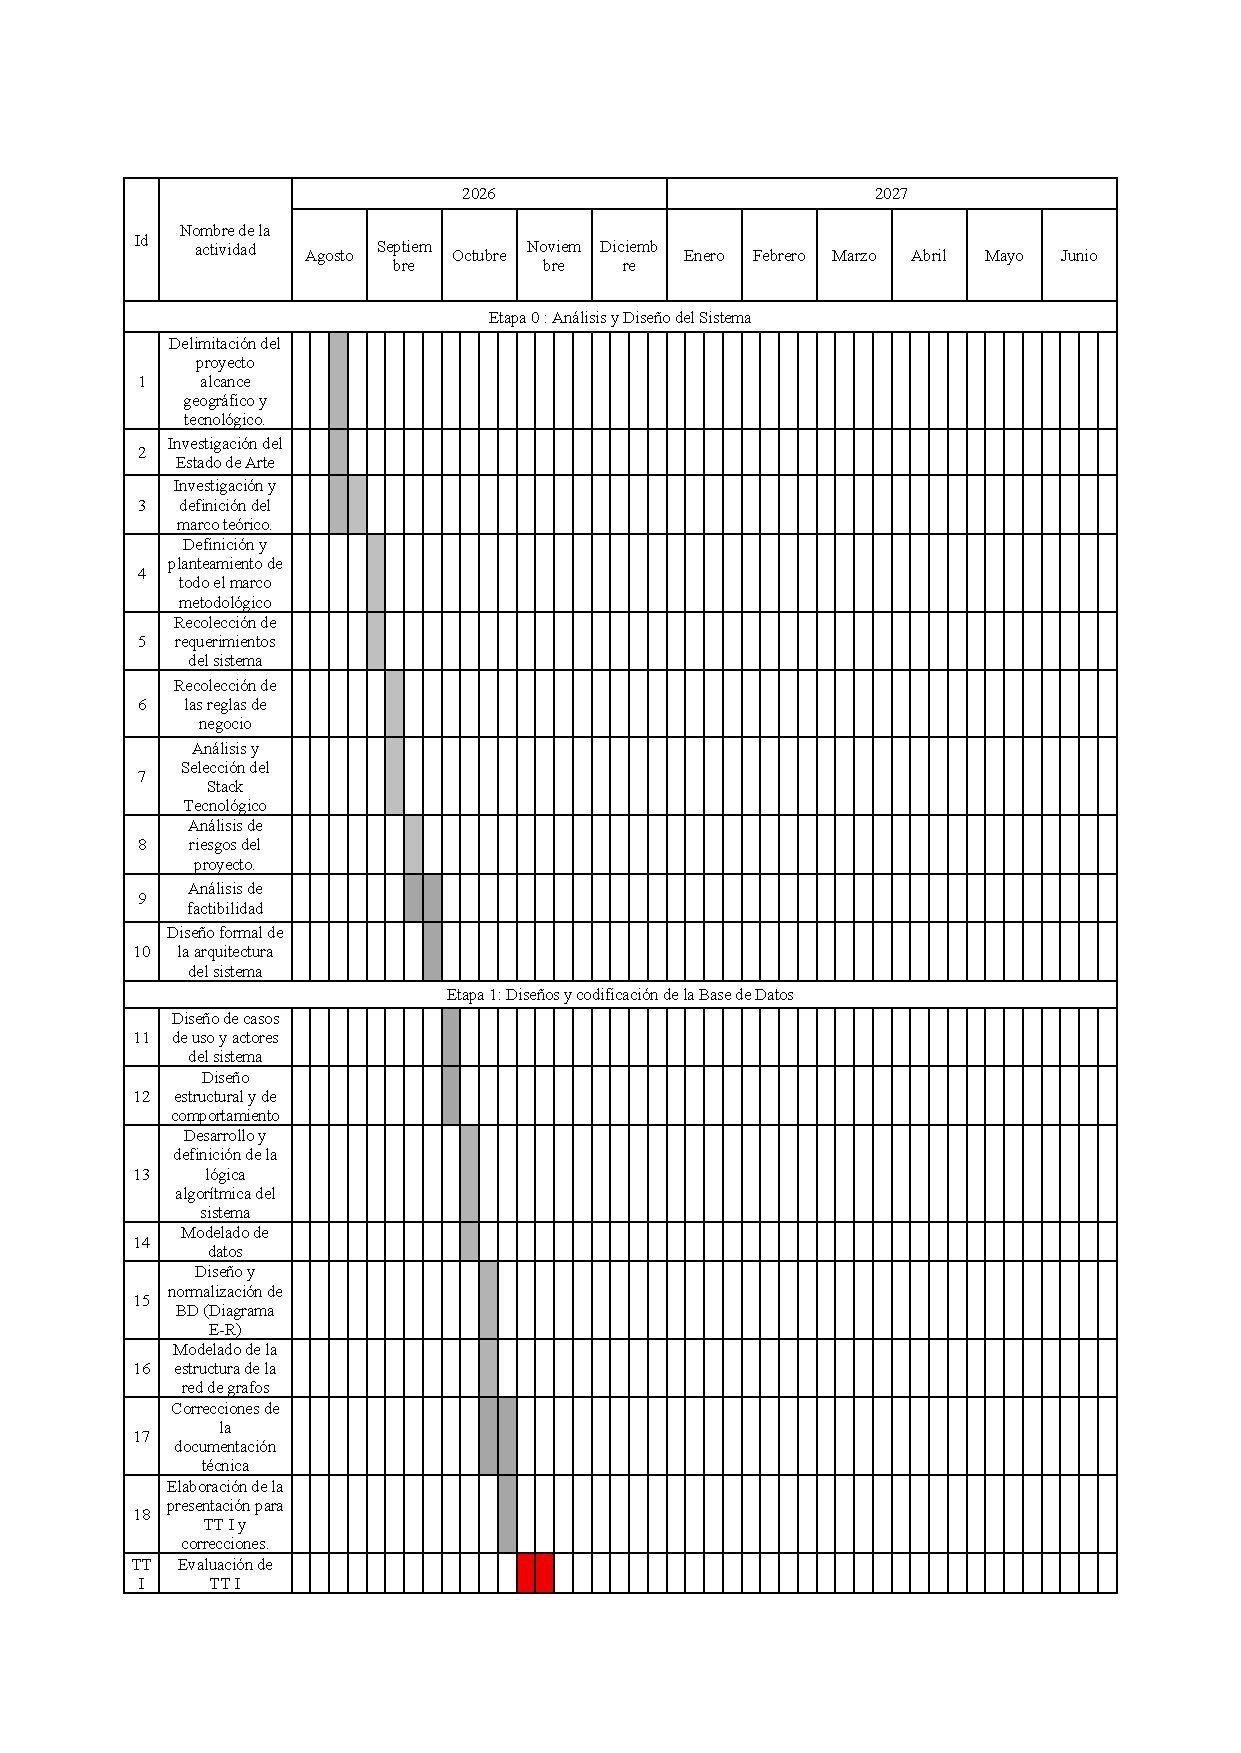
\includegraphics[width=\textwidth, trim={2cm 2cm 2cm 3cm}, clip]{figures/capitulo5_analisis_sistema/5.5_Analisis_de_Factibilidad/Cronograma_2027_TT1.pdf} 
    \caption{Diagrama de Gantt general de actividades del Trabajo Terminal}
    \label{fig:cronograma_actividades}
\end{figure}

\begin{figure}[H]
    \centering
    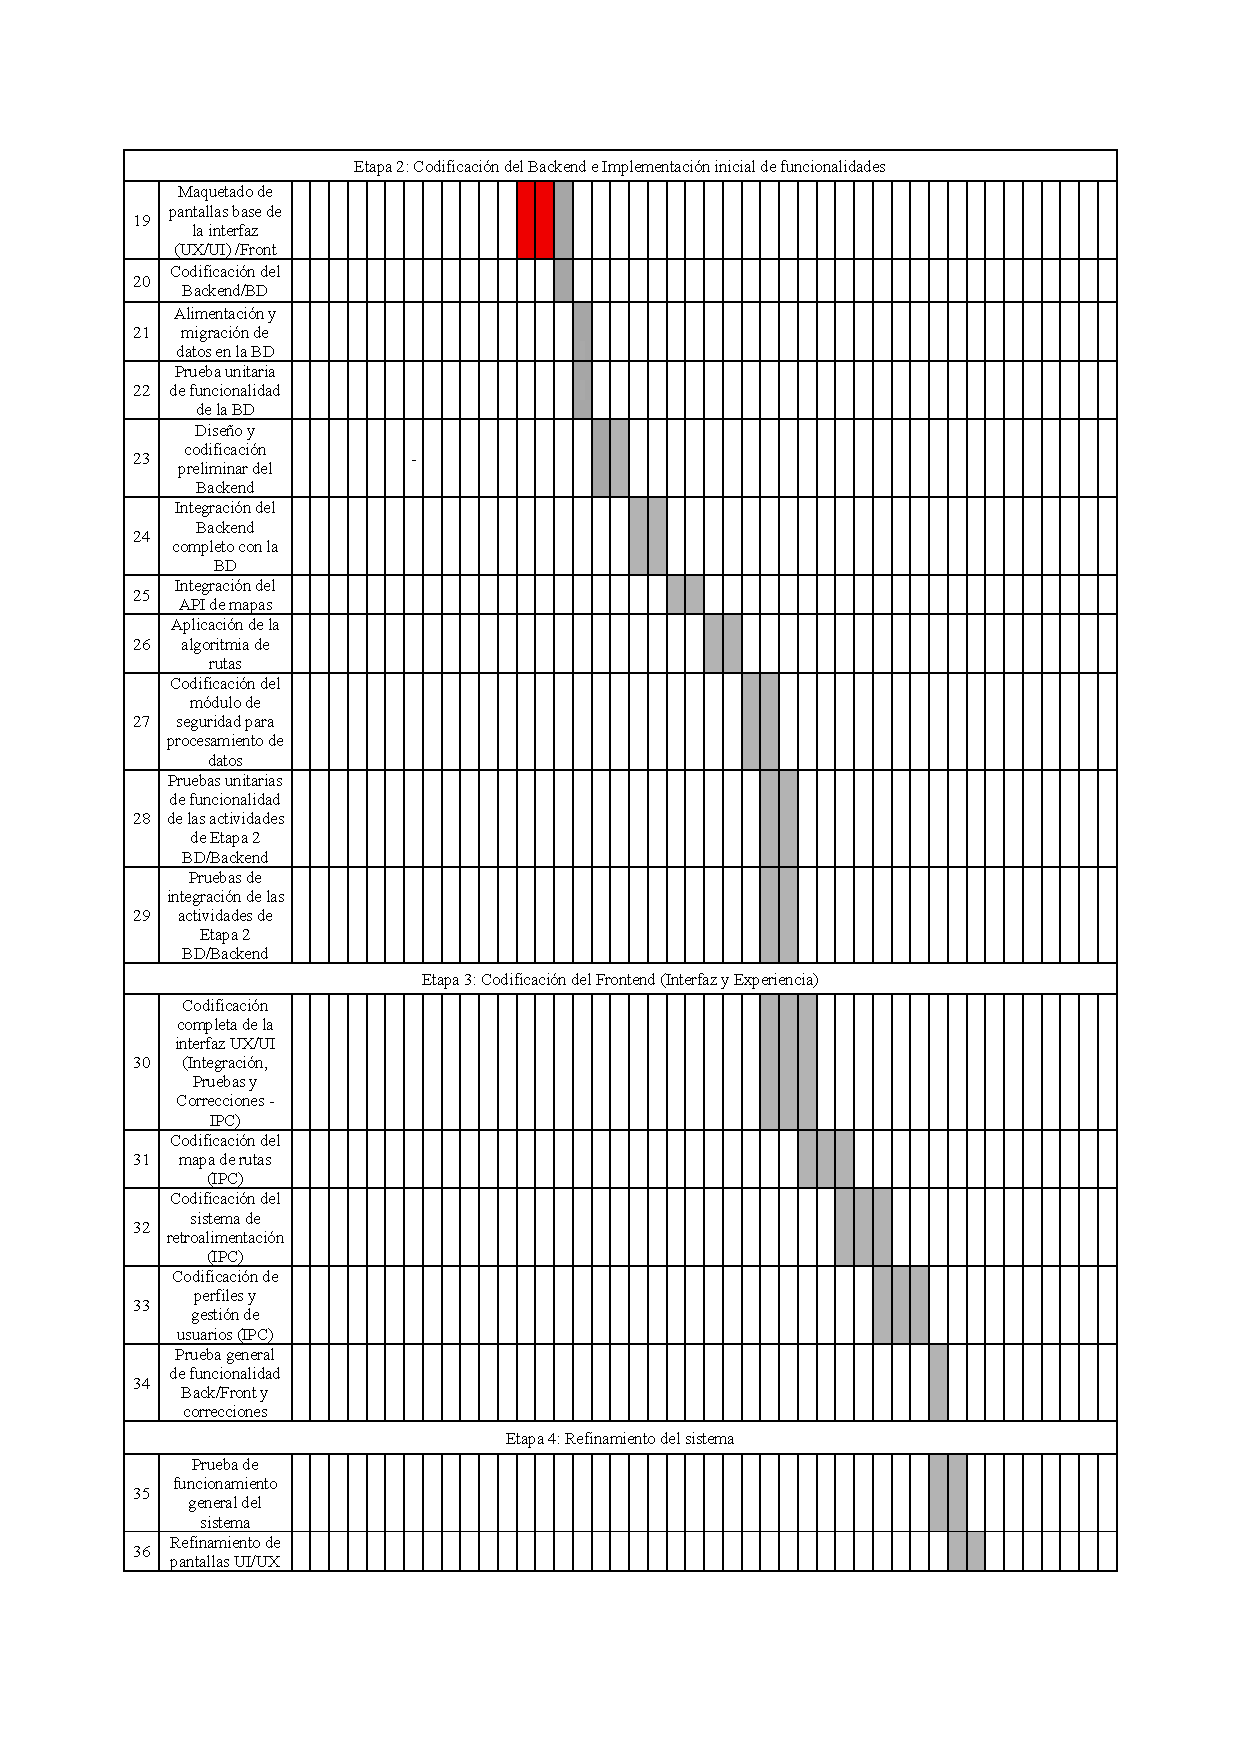
\includegraphics[width=\textwidth, trim={2cm 2cm 2cm 3cm}, clip]{figures/capitulo5_analisis_sistema/5.5_Analisis_de_Factibilidad/Cronograma_2027_TT1-1-2-2.pdf} 
    \caption*{Continuación del diagrama \ref{fig:cronograma_actividades}}
\end{figure}

\begin{figure}[H]
    \centering
    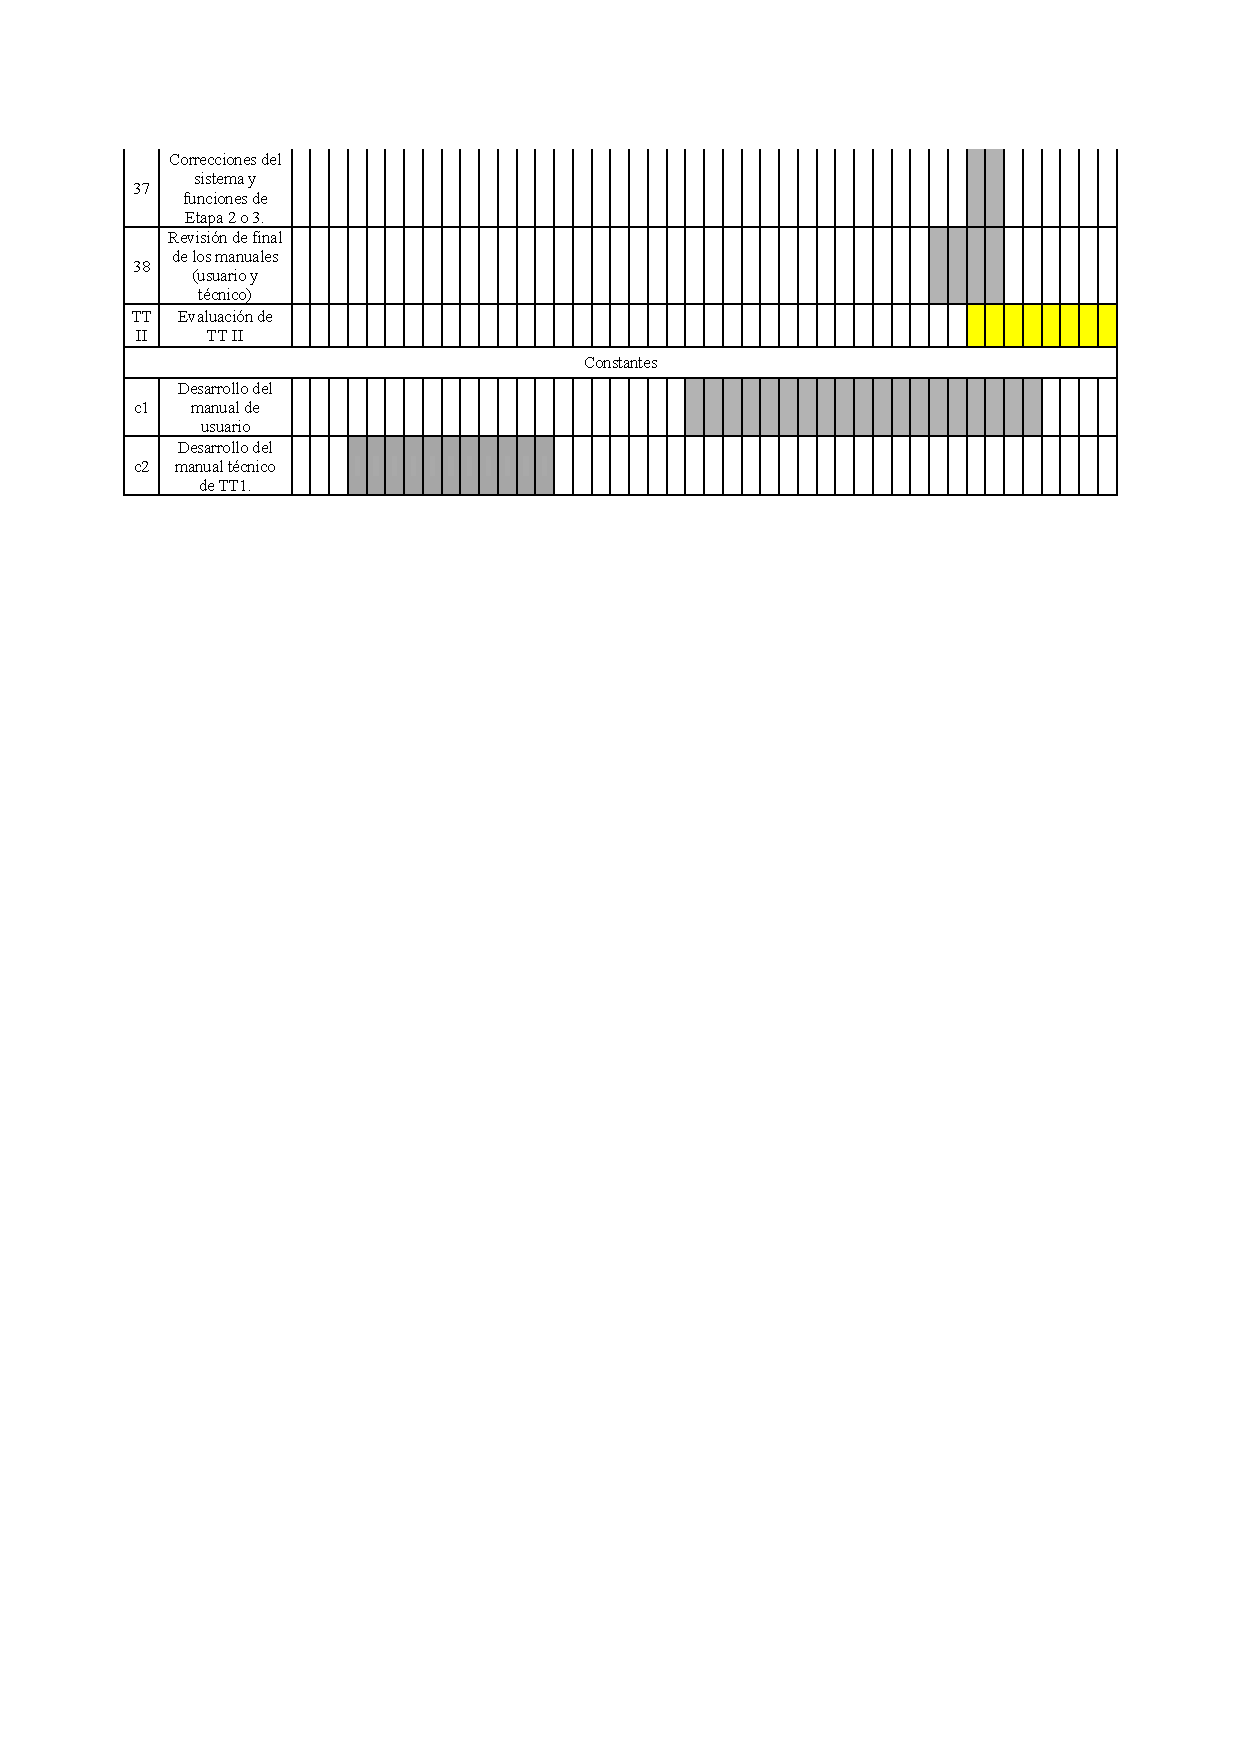
\includegraphics[width=\textwidth, trim={2cm 21cm 2cm 2cm}, clip]{figures/capitulo5_analisis_sistema/5.5_Analisis_de_Factibilidad/Cronograma_2027_TT1-3.pdf} 
    \caption*{Continuación del diagrama \ref{fig:cronograma_actividades}}
\end{figure}

Es necesario realizar la comparación entre el diagrama de Gantt (plazos definidos) contra el tiempo real requerido para el proyecto, de esta forma se observa si realmente el sistema es factible dentro de los intervalos de tiempo establecidos.

En la tabla \ref{tab:resumen_dias} se calcula el tiempo de esfuerzo requerido en base a la cantidad de horas de trabajo que el equipo invierte en el sistema obteniendo la cantidad de días laborales (tomando en cuenta una jornada de tiempo completo; 8 horas) necesarios para el desarrollo dentro del intervalo general de tiempo. 

El plazo de trabajo parte en la tercera semana de Agosto de 2026 y finaliza hasta mediados de Mayo del 2027, considerando que las fechas de presentación de TT I-II se realizan aproximadamente un mes antes de la finalización del periodo escolar. 

\begin{table}[H]
\centering
\renewcommand{\arraystretch}{1.2}
\resizebox{\textwidth}{!}{
\begin{tabular}{l c c c c c c c}
\hline
\textbf{Mes} & \textbf{Días} & \textbf{\makecell{Fin de\\semana}} & \textbf{\makecell{Días no\\laborales}} & \textbf{\makecell{Días\\hábiles}} & \textbf{\makecell{Horas de\\trabajo\\por día\\(promedio)}} & \textbf{\makecell{Horas\\totales}} & \textbf{\makecell{Días\\laborales\\(8 horas\\al día)}} \\ \hline
\textbf{Agosto} & 15 & 4 & 0 & 11 & 4 & 44 & 5.5 \\ 
\textbf{Septiembre} & 30 & 8 & 1 & 21 & 4 & 84 & 10.5 \\ 
\textbf{Octubre} & 31 & 9 & 0 & 22 & 4 & 88 & 11 \\ 
\textbf{Noviembre} & 30 & 9 & 2 & 19 & 4 & 76 & 9.5 \\ 
\textbf{Diciembre} & 30 & 8 & 0 & 22 & 4 & 88 & 11 \\ 
\textbf{Enero} & 31 & 10 & 1 & 20 & 4 & 80 & 10 \\ 
\textbf{Febrero} & 28 & 8 & 1 & 19 & 4 & 76 & 9.5 \\ 
\textbf{Marzo} & 31 & 8 & 3 & 20 & 4 & 80 & 10 \\ 
\textbf{Abril} & 30 & 8 & 5 & 17 & 4 & 68 & 8.5 \\ 
\textbf{Mayo} & 31 & 10 & 2 & 19 & 4 & 76 & 9.5 \\ 
\textbf{Junio} & 7 & 2 & 0 & 5 & 4 & 20 & 2.5 \\ \hline
\textbf{Total} & \textbf{294} & \textbf{84} & \textbf{15} & \textbf{195} & & \textbf{780} & \textbf{97.5} \\ \hline
\end{tabular}
} 
\caption{Resumen de días para el desarrollo del proyecto (Agosto 2026 - Junio 2027) con base a los plazos establecidos en el Diagrama de Gantt \ref{fig:cronograma_actividades}.}
\label{tab:resumen_dias}
\end{table}

Como se aprecia en la tabla \ref{tab:resumen_dias} se cuentan con aproximadamente 98 días laborales para el desarrollo del trabajo terminal considerando una jornada laboral de 8 días, eliminando días festivos, fines de semana y periodos que no entran en el intervalo de tiempo.

%Pendiente por desarrollar el calculo del tiempo real con formulas matematicas de cada actividad para la estimacion real de esfuerzo en tiempo requerido y el contraste con los plazos ya definidos.                                                                                                                                                                                                                            




\subsection{Factibilidad económica}
\label{sec:factibilidad_economica}
A continuación se presenta el análisis de costos asociados al desarrollo del prototipo de aplicación móvil. Los costos de recursos humanos se calculan con base en tarifas de mercado vigentes para cada rol, con el fin de dimensionar el valor económico del trabajo invertido. Por otra parte, los recursos tecnológicos sí representan egresos reales derivados del uso de servicios externos necesarios para el preprocesamiento de datos del sistema. Todos los costos se expresan en pesos mexicanos (MXN) y se acompañan de la fuente y fecha de consulta correspondiente.

\paragraph{Recursos humanos}

Para la realización del proyecto se contempla la participación del equipo de trabajo terminal, compuesto por tres integrantes que colaboran de manera conjunta en todas las etapas del desarrollo, especializándose respectivamente en el diseño y construcción de la base de datos y la lógica algorítmica, el desarrollo de la aplicación móvil, y el análisis y tratamiento de los datos geoespaciales y delictivos. Dado que el proyecto se desarrolla bajo la metodología Scrumban, las funciones de coordinación del equipo son rotativas entre sus integrantes y se ejercen dentro del mismo horario de trabajo individual, por lo que no representan un costo adicional de recursos humanos.

Se considera una dedicación de 2 horas diarias por integrante a lo largo del periodo efectivo de desarrollo del proyecto, comprendido entre el 24 de agosto de 2026 y mediados de mayo de 2027 (aproximadamente 9 meses) conforme al cronograma de actividades. De acuerdo con el Calendario Escolar 2026-2027 del Instituto Politécnico Nacional \cite{ipn_calendario2026}, el cálculo de días hábiles efectivos se obtiene de la siguiente manera:

\begin{align*}
\text{Días hábiles totales (24 ago. 2026 -- 15 may. 2027)} &= 190 \\
(-)\ \text{Días festivos (descanso obligatorio y acuerdo sindical)} &= 12 \\
(-)\ \text{Periodos vacacionales (dic.--ene. y mar.--abr.)} &= 22 \\
\hline
\text{Días hábiles efectivos} &= 156
\end{align*}

\[
156 \text{ días} \times 2 \text{ horas/día} = 312 \text{ horas efectivas por integrante}
\]

La Tabla~\ref{tab:sueldos_mercado} presenta el sueldo mensual promedio en México para cada rol del equipo, obtenido de fuentes de empleo consultado el 6 de octubre del 2026.

\begin{table}[H]
    \centering
    \caption[Sueldo mensual promedio por rol]{Sueldo mensual promedio por rol, según datos de mercado.}
    \vspace{0.2cm}
    \resizebox{\textwidth}{!}{%
    \begin{tabular}{|l|l|c|}
        \hline
        \textbf{Cargo} & \textbf{Fuente} & \textbf{Sueldo mensual promedio} \\ \hline
        Backend Developer & Indeed México \cite{indeed_backend_developer} & \$ 19,210.00 \\ \hline
        Analista de Datos & Indeed México \cite{indeed_analistas_datos} & \$ 15,221.00 \\ \hline
        Desarrollador Móvil & Indeed México \cite{indeed_android_developer} & \$ 17,302.00 \\ \hline
    \end{tabular}%
    }
    \label{tab:sueldos_mercado}
\end{table}

El costo por hora de cada rol se obtiene dividiendo el sueldo mensual promedio entre 160 horas mensuales, correspondientes a una jornada estándar de 8 horas diarias durante 20 días hábiles al mes. Este costo por hora se multiplica por las 312 horas efectivas estimadas por integrante, obteniendo el costo total de recursos humanos mostrado en la Tabla~\ref{tab:recursos_humanos}.

\begin{table}[H]
    \centering
    \caption[Recursos humanos necesarios para realizar el proyecto]{Recursos humanos necesarios para realizar el proyecto. Elaboración propia.}
    \vspace{0.2cm}
    \resizebox{\textwidth}{!}{%
    \begin{tabular}{|l|c|c|c|}
        \hline
        \textbf{Cargo} & \textbf{Horas estimadas} & \textbf{Costo/hora} & \textbf{Costo total} \\ \hline
        Backend Developer & 312 & \$ 120.06 & \$ 37,458.72 \\ \hline
        Analista de Datos & 312 & \$ 95.13 & \$ 29,680.56 \\ \hline
        Desarrollador Móvil & 312 & \$ 108.14 & \$ 33,739.68 \\ \hline
        \multicolumn{3}{|r|}{\textbf{Total}} & \textbf{\$ 100,878.96} \\ \hline
    \end{tabular}%
    }
    \label{tab:recursos_humanos}
\end{table}


\paragraph{Recursos tecnológicos}

Para la realización del proyecto se contempla el uso de los siguientes recursos de hardware, software y servicios en la nube. El equipo de cómputo empleado es propiedad de los integrantes del equipo, por lo que no representa un costo de adquisición adicional para el proyecto. El consumo eléctrico y de internet asociado a su uso durante el desarrollo se contabiliza por separado en la sección de Recursos materiales. Para el desarrollo de la aplicación móvil se emplea el framework Flutter (Dart), mientras que para la gestión de la base de datos y el motor de ruteo geoespacial se utiliza Supabase (PostgreSQL con las extensiones PostGIS y pgRouting), justificado técnicamente en la sección~\ref{sec:factibilidad_técnica}.

El plan gratuito de Supabase ofrece 500 MB de base de datos, 500 MB de almacenamiento de archivos, 5 GB de transferencia de datos mensual y solicitudes de API ilimitadas \cite{supabase_pricing}. El polígono de estudio delimitado en la Figura~\ref{fig:mapa_zona_estudio} abarca una superficie de 26.31 km\textsuperscript{2} y su red vial comprende aproximadamente 11{,}700 segmentos de calle. Considerando un peso promedio de 1 a 3 KB por segmento, el volumen estimado de la base de datos se ubica entre 12 y 35 MB, muy por debajo del límite mencionado, por lo que se opta por el plan gratuito.

Para el preprocesamiento de la información se emplea la Street View Static API de Google Maps Platform, mediante la cual se obtendrán tres imágenes por cada segmento de calle, es decir, aproximadamente 35{,}100 solicitudes. Esta API ofrece una cuota gratuita de 10{,}000 solicitudes mensuales y cobra \$7.00 USD por cada 1{,}000 solicitudes adicionales \cite{google_maps_pricing}, por lo que se generarían 25{,}100 solicitudes facturables, equivalentes a \$175.70 USD (\$3,156.80 MXN). Posteriormente, las imágenes se analizan con el modelo Qwen3.7-Flash \cite{qwen_pricing}, cuyo costo para solicitudes de hasta 32{,}000 tokens es de \$0.03 USD por millón de tokens de entrada y \$0.13 USD por millón de tokens de salida. Considerando un consumo aproximado de 2{,}000 tokens de entrada y 500 de salida por imagen, el análisis de las 35{,}100 imágenes requiere 70.2 millones de tokens de entrada y 17.55 millones de salida, con un costo total de \$4.39 USD (\$78.83 MXN). Durante la operación de la aplicación se utiliza el SDK de Maps para dispositivos móviles, cuyo uso es ilimitado y sin costo, y Places API (New), cuyas SKU de Autocomplete y Place Details Essentials incluyen 10{,}000 solicitudes gratuitas mensuales cada una \cite{google_maps_pricing}. Los montos expresados en dólares estadounidenses se convirtieron a pesos mexicanos con el tipo de cambio FIX publicado por el Banco de México el 6 de octubre de 2026, equivalente a \$17.9670 MXN por dólar \cite{banxico_fix}.

Adicionalmente, el equipo utiliza dos servicios por suscripción mensual durante el desarrollo del proyecto: Overleaf, para la redacción del documento en LATEX, y Udemy, para la capacitación técnica de los integrantes. Considerando una duración de nueve meses, el costo de estos servicios se desglosa en la Tabla~\ref{tab:servicios_adicionales}.

El proyecto contempla como entregable un prototipo funcional de la aplicación móvil, cuya conclusión no depende de su publicación en una tienda de aplicaciones. No obstante, de presentarse la oportunidad, el prototipo podrá publicarse en Google Play Store, lo que requiere un pago único de registro de desarrollador de \$25.00 USD (\$449.18 MXN) \cite{google_play_console}. Al tratarse de un gasto opcional, no se incluye en el total del presupuesto.

\begin{table}[H]
    \centering
    \caption[Recursos tecnológicos necesarios para realizar el proyecto]{Recursos tecnológicos necesarios para realizar el proyecto. Elaboración propia.}
    \vspace{0.2cm}
    \resizebox{\textwidth}{!}{%
    \begin{tabular}{|l|l|c|}
        \hline
        \textbf{Cantidad} & \textbf{Descripción} & \textbf{Costo} \\ \hline
        \multicolumn{3}{|l|}{\textit{Hardware}} \\ \hline
        3 & Equipo de cómputo propio del equipo & \$ 0.00 \\ \hline
        \multicolumn{3}{|l|}{\textit{Software y servicios en la nube}} \\ \hline
        1 & Flutter / Dart (código abierto) & \$ 0.00 \\ \hline
        1 & Supabase -- plan gratuito (PostgreSQL, PostGIS, pgRouting) & \$ 0.00 \\ \hline
        1 & Git / GitHub (plan gratuito) & \$ 0.00 \\ \hline
        1 & Google Meet (plan gratuito) & \$ 0.00 \\ \hline
        1 & Notion (plan estudiante, gratuito) & \$ 0.00 \\ \hline
        \multicolumn{3}{|l|}{\textit{APIs de preprocesamiento (35{,}100 imágenes: 11{,}700 segmentos $\times$ 3)}} \\ \hline
        35{,}100 & Google Street View Static API (10{,}000 gratuitas; 25{,}100 a \$7.00 USD/1{,}000) & \$ 3,156.80 \\ \hline
        35{,}100 & Qwen3.7-Flash, análisis de imágenes (70.2 M tokens de entrada y 17.55 M de salida) & \$ 78.83 \\ \hline
        \multicolumn{3}{|l|}{\textit{APIs de operación de la aplicación}} \\ \hline
        1 & Maps SDK para móvil (uso ilimitado sin costo) & \$ 0.00 \\ \hline
        1 & Places API (New), dentro de la cuota gratuita & \$ 0.00 \\ \hline
        \multicolumn{3}{|l|}{\textit{Opcional (no incluido en el total)}} \\ \hline
        1 & Registro de desarrollador Google Play (pago único) & \$ 449.18 \\ \hline
        \multicolumn{2}{|r|}{\textbf{Total}} & \textbf{\$ 3,235.63} \\ \hline
    \end{tabular}%
    }
    \label{tab:recursos_tecnologicos}
\end{table}

\begin{table}[H]
    \centering
    \caption[Servicios adicionales por suscripción mensual]{Servicios adicionales por suscripción mensual. Elaboración propia.}
    \vspace{0.2cm}
    \resizebox{\textwidth}{!}{%
    \begin{tabular}{|c|l|c|c|}
        \hline
        \textbf{Meses} & \textbf{Descripción} & \textbf{Costo mensual} & \textbf{Costo total} \\ \hline
        9 & Overleaf (suscripción mensual) & \$ 99.00 & \$ 891.00 \\ \hline
        9 & Udemy (suscripción mensual) & \$ 209.00 & \$ 1,881.00 \\ \hline
        \multicolumn{3}{|r|}{\textbf{Total}} & \textbf{\$ 2,772.00} \\ \hline
    \end{tabular}%
    }
    \label{tab:servicios_adicionales}
\end{table}

\paragraph{Recursos materiales}

Para la realización del proyecto se contemplan los siguientes recursos materiales asociados a la operación básica del equipo de trabajo. El costo de la energía eléctrica se estima a partir del consumo de los equipos de cómputo durante las horas efectivas de trabajo. Considerando las 312 horas efectivas por integrante calculadas en la sección de recursos humanos, y una potencia aproximada de 65 W por equipo, el consumo se obtiene de la siguiente manera:

\begin{align*}
\text{Horas de uso} &= 312 \text{ h} \times 3 \text{ integrantes} = 936 \text{ h} \\
\text{Consumo} &= 936 \text{ h} \times 0.065 \text{ kW} = 60.84 \text{ kWh} \approx 61 \text{ kWh}
\end{align*}

Dicho consumo se valora con la cuota del consumo excedente de la Tarifa 1 de la Comisión Federal de Electricidad para octubre de 2026, equivalente a \$4.054 por kilowatt-hora \cite{cfe_tarifa1}, considerada como valor conservador. Respecto al servicio de internet, cada integrante cuenta con un paquete residencial de 100 Mbps con costo mensual de \$390.00 \cite{totalplay_paquetes}, el cual se contabiliza durante los 9 meses de desarrollo del proyecto.

\begin{table}[H]
    \centering
    \caption[Recursos materiales necesarios para realizar el proyecto]{Recursos materiales necesarios para realizar el proyecto. Elaboración propia.}
    \vspace{0.2cm}
    \resizebox{\textwidth}{!}{%
    \begin{tabular}{|l|l|c|c|}
        \hline
        \textbf{Cantidad} & \textbf{Descripción} & \textbf{Costo} & \textbf{Total} \\ \hline
        61 & Energía eléctrica, Tarifa 1 CFE (kWh) & \$ 4.054 & \$ 247.29 \\ \hline
        27 & Internet residencial 100 Mbps (3 integrantes $\times$ 9 meses) & \$ 390.00 & \$ 10,530.00 \\ \hline
        \multicolumn{3}{|r|}{\textbf{Total}} & \textbf{\$ 10,777.29} \\ \hline
    \end{tabular}%
    }
    \label{tab:recursos_materiales}
\end{table}


\paragraph{Flujo de pago}

El costo total estimado del proyecto se resume en la Tabla~\ref{tab:flujo_pago} y asciende a \$129,430.27 MXN, que resulta de sumar los recursos humanos, tecnológicos y materiales (\$117,663.88 MXN) y un 10\% de imprevistos calculado sobre dicho subtotal (\$11,766.39 MXN). No se considera el pago opcional de registro en Google Play Store. De este monto, \$100,878.96 corresponden al valor de mercado del trabajo del equipo, el cual, al ser realizado directamente por los integrantes del trabajo terminal sin una relación de contratación formal, no representa un desembolso. De igual forma, los recursos materiales (energía eléctrica e internet) corresponden a servicios que los integrantes ya tienen contratados, por lo que se contabilizan para dimensionar el costo real del proyecto sin implicar un gasto adicional. En consecuencia, el egreso efectivo se limita a los recursos tecnológicos, por un monto de \$6,007.63 MXN, equivalente a aproximadamente \$2,002.54 MXN por integrante a lo largo de los nueve meses de desarrollo (\$222.50 MXN mensuales).

Con base en lo anterior, el proyecto se considera económicamente viable: el gasto efectivo es reducido y proviene principalmente de servicios de preprocesamiento de uso único y de suscripciones mensuales, mientras que el resto de los costos corresponde a trabajo y recursos que el equipo ya posee o tiene contratados.

\begin{table}[H]
    \centering
    \caption[Resumen de costos totales del proyecto]{Resumen de costos totales del proyecto. Elaboración propia.}
    \vspace{0.2cm}
    \begin{tabular}{|l|c|}
        \hline
        \textbf{Recursos} & \textbf{Costo} \\ \hline
        Recursos Humanos & \$ 100,878.96 \\ \hline
        Recursos Tecnológicos & \$ 6,007.63 \\ \hline
        Recursos Materiales & \$ 10,777.29 \\ \hline
        Subtotal & \$ 117,663.88 \\ \hline
        Imprevistos (10\%) & \$ 11,766.39 \\ \hline
        \textbf{Total} & \textbf{\$ 129,430.27} \\ \hline
    \end{tabular}
    \label{tab:flujo_pago}
\end{table}

\subsection{Factibilidad legal}
\label{sec:factibilidad_legal}
En este apartado se analiza la factibilidad legal del proyecto, donde se verifica el cumplimiento de los requisitos jurídicos y si esta dentro de las leyes, normas y reglamentos vigentes del marco jurídico sin llegar a infringir leyes, derechos de autor o licencias de terceros.  



\subsection{Factibilidad de recursos}
\label{sec:factibilidad_recursos}
\input{documents/capitulo5_analisis_sistema/5.5_Analisis_de_Factibilidad/5.5.5_Factibilidad_recursos/seccion5_5_5}




